\chapter{Theory and motivation}
\label{chap:theory}
To understand and motivate the searches presented in chapters 
\ref{chap:hhh} and \ref{chap:mssm} it is important
to understand the theory and phenomenology behind them. 
This chapter describes the \acl{SM} of particle physics, the
motivations for \acl{SUSY} and the phenomenology of Higgs
sectors beyond the \acl{SM}.

\section{The \acl{SM} of particle physics}
\label{sec:theory_sm}
The \ac{SM} of particle physics is a theory that describes the weak and strong
nuclear forces, plus the \ac{EM} force, and the interaction of those forces
with particles. The \ac{SM} is a \ac{QFT} in which matter particles
are represented by spin-$\frac{1}{2}$ fermions, with the forces represented
by spin-1 bosons.

\subsection{Fundamental particles and forces}
\label{sec:theory_sm_particles}
In the \ac{SM} there are twelve fundamental fermions, six quarks and
six leptons. The quarks interact via both strong nuclear force and the 
electroweak force, while
the leptons only interact via the electoweak force.
Each of the fermions has a corresponding antiparticle
with opposite quantum numbers. The quarks and leptons
are divided into three generations. The particles from different
generations have similar properties, apart from the mass which increases
for each generation. The quarks and leptons are summarised in 
table \ref{tab:theory_fermions}.

\begin{table}[htp]
\begin{center}
\caption{The fundamental fermions}
\begin{tabular}{@{}llll@{}}
\toprule
 & \textbf{1st generation} & \textbf{2nd generation} & \textbf{3d generation}\\
\midrule
\textbf{Quarks} & & & \\
\midrule
Charge: +$\frac{2}{3}$& up (\Pup)  & charm (\Pcharm) & top (\Ptop) \\
Charge: -$\frac{1}{3}$& down (\Pdown) & strange (\Pstrange) & bottom (\Pbottom) \\
\midrule
\textbf{Leptons} & & & \\
\midrule
Charge: -1 & electron (\Pe) & muon (\Pgm) & tau (\Pgt) \\
Charge: 0  & electron neutrino ($\Pgn_{\Pe}$) & muon neutrino ($\Pgn_{\Pgm}$) & tau neutrino ($\Pgn_{\Pgt}$)\\
\bottomrule
\end{tabular}
\label{tab:theory_fermions}
\end{center}
\end{table}

The forces in the \ac{SM} are mediated by spin-1 bosons: The gluon (\Pgluon),
which carries the strong force, the photon (\Pphoton) as the
electromagnetic force carrier, and the $\PW^{\pm}$ and \PZ bosons, the
force carriers of the weak nuclear force. 

The particles that interact via the strong force carry colour charge (red, green, or blue),
as do their mediators, the gluons. The interactions in the \ac{QFT} of the
strong force, called \ac{QCD}, are governed by an SU(3) (colour) symmetry.
%There are 8 gluons due to the SU(3) symmetry, colour octet and a colour singlet, but
%if there was a colour singlet it should occur as a free particle while it does not.
%See chapter 285 of griffiths
The quarks are never observed in isolation but always in bound
hadron states, which is referred to as confinement. Due to asymptotic
freedom \cite{asympt-I,asympt-II}, the strong coupling strength decreases at 
high energy (short distances). More detailed introductions to \ac{QCD} can 
be found in ref. \cite{griffiths}.

Particles that carry electric charge interact via the 
electromagnetic force, summarised in by the rules of \ac{QED}. 
The weak interaction, governed by weak isospin transformations,
only couples to the left-handed part of the fermion states. In 
general a fermion state can be decomposed into its left- and right-handed parts
\begin{equation}\label{eqn:leftright}
\chi=\psi_R+\psi_L,
\end{equation}
and only $\psi_L$ will interact via the weak force. Handedness and
helicity have the same eigenstates for massless particles, and as
such neutrinos, which are massless in the \ac{SM}, must all be left-handed.
The observation of neutrino flavour oscillations since the formulation of
the \ac{SM} implies that neutrinos do have a small but finite mass
and so there must be right-handed neutrinos in the \ac{SM}. This is
not discussed further here ADD REFERENCE.
The weak isospin acts on doublets of left-handed lepton pairs, while
the right-handed leptons transform as singlet states. This works similarly
for the quarks, with weak isospin acting three left-handed doublets and
six right-handed singlets. Note that the weak eigenstates of the quarks
differ from the physical states, which mix via the \ac{CKM}-matrix CITATION
in charged current interactions as
\begin{equation}\label{eqn:ckm_matrix}
\begin{pmatrix} d' \\
s' \\
b'  \end{pmatrix} = \begin{pmatrix} V_{ud} & V_{us} & V_{ub} \\
V_{cd} & V_{cs} & V_{cb} \\
V_{td} & V_{ts} & V_{tb} \end{pmatrix} \begin{pmatrix} d \\
s\\
b \end{pmatrix}.
\end{equation}

\subsection{The electroweak force}
\label{sec:theory_sm_ewk}
The unification of the weak and electromagnetic forces, introduced
in the 1960s by Glashow \cite{glashow-ewk}, Weinberg \cite{weinberg-ewk} and Salam \cite{salam-ewk},
is a key component of the \ac{SM}. The unification of these forces,
governed by an SU(2)$\times$U(1) symmetry, implies the presence of a charged
current. A quantum number, weak hypercharge $Y$, is introduced. Weak
hypercharge is related to weak isospin $I_{1,2,3}$ and electric charge as
\begin{equation}\label{eqn:hypercharge}
Q=I_3 + \frac{1}{2}Y.
\end{equation}
We then have the three weak isospin fields, $W_{\mu}^{i}$, and the
weak hypercharge field $Y_{\mu}$, which mix to form the physical \Pphoton,
\PZ and $\PW^{\pm}$ states as
\begin{align}\label{eqn:ewk_propagators}
\PW^{\pm} &= \frac{1}{\sqrt{2}}(W_{\mu}^1 \mp i W_{\mu}^2),\\
A_{\mu} &= W_{\mu}^3\sin{\theta_W} + Y_{\mu}\cos{\theta_W},\\
Z_{\mu} &= W_{\mu}^3\cos{\theta_W} - Y_{\mu}\sin{\theta_W}.
\end{align}
In these equations $A_{\mu}$ is the photon field and $Z_{\mu}$ the \PZ field.
The weak mixing angle $\theta_W$ is related to the weak (g) and electromagnetic (g')
coupling constants as
\begin{equation}\label{eqn:thetaw}
g\sin{\theta_W} = g'\cos{\theta_W}
\end{equation}

The gauge invariance of the Lagrangian would be broken
by the addition of mass terms. For the photon this is fine, as we know it
is massless, but it is known that the \PW and \PZ bosons, as well as fermions, 
are massive. This means electroweak symmetry must be broken. In the \ac{SM}
this is achieved via the Higgs mechanism.

\subsection{The Higgs mechanism}
\label{sec:theory_sm_higgsmech}
The masses of the vector bosons are generated via the
Higgs mechanism, proposed in the 1960s by Englert and Brout \cite{englertbrout}

\section{Standard model Higgs boson measurements}
\label{sec:theory_smH}
The mass of the Higgs boson is a free parameter in the \ac{SM}, and so
searches for the boson had to be conducted over a large range of
masses. Searches for the Higgs boson at \ac{LEP} did not lead
to its observation. However, masses below 114.4 GeV were excluded at 95\% \ac{CL} \cite{LEP-Higgs},
providing a lower search limit. Subsequent studies at the 
Tevatron did also not lead to discovery of the Higgs boson, but did provide
an additional excluded masses range of 140-186 GeV at 95\% \ac{CL} \cite{TEV-Higgs}.

On the fourth of July 2012 the ATLAS and CMS collaborations
announced the discovery of a boson with a mass of around 125 GeV \cite{HDiscoveryATLAS,HDiscoveryCMS}.
The observations were based on excesses in the search for $\PHiggslight\rightarrow\gamma\gamma$ and $\PHiggslight\rightarrow \PZ\PZ$.
More data were collected and analysed during the remainder of 2012, and subsequent studies 
grew the confidence in this boson being compatible with the standard model Higgs boson. The ATLAS and CMS combined
mass measurement using the full dataset of Run 1 of the \ac{LHC} 
found \mh = $125.09 \pm 0.21 \text{ (stat) } \pm 0.11 \text{ (syst) }$ GeV \cite{MassComb}.
The combined ATLAS and CMS production- and decay rate measurement, also using the full dataset of \ac{LHC} Run 1,
shows very good agreement with the \ac{SM} predictions \cite{CouplComb}. In addition, through
this combination the $\PHiggslight \rightarrow \Pgt\Pgt$ decay was observed with a significance of 5.5$\sigma$, while
the individual experiments did not reach a significance upwards of 5$\sigma$ in this channel during Run 1.
Despite the good agreement with the \ac{SM}, some discrepancies do remain, 
and so the measurements of \ac{SM} Higgs boson
properties are certainly not finished yet.

\begin{figure}[h!]
\begin{center}
\subfloat[Gluon fusion]{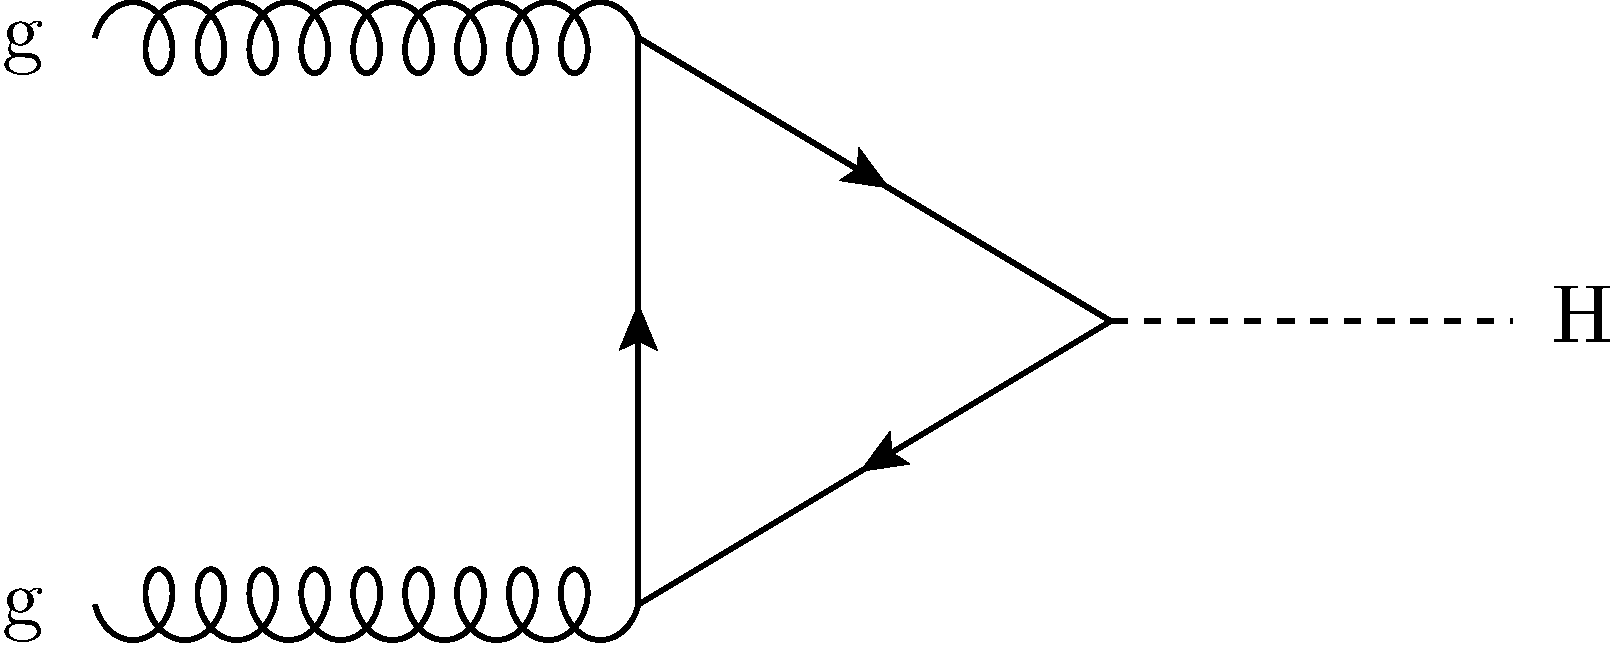
\includegraphics[width=0.5\textwidth]{./Theory/Figures/feynman_ggH.pdf}}
\subfloat[Vector boson fusion]{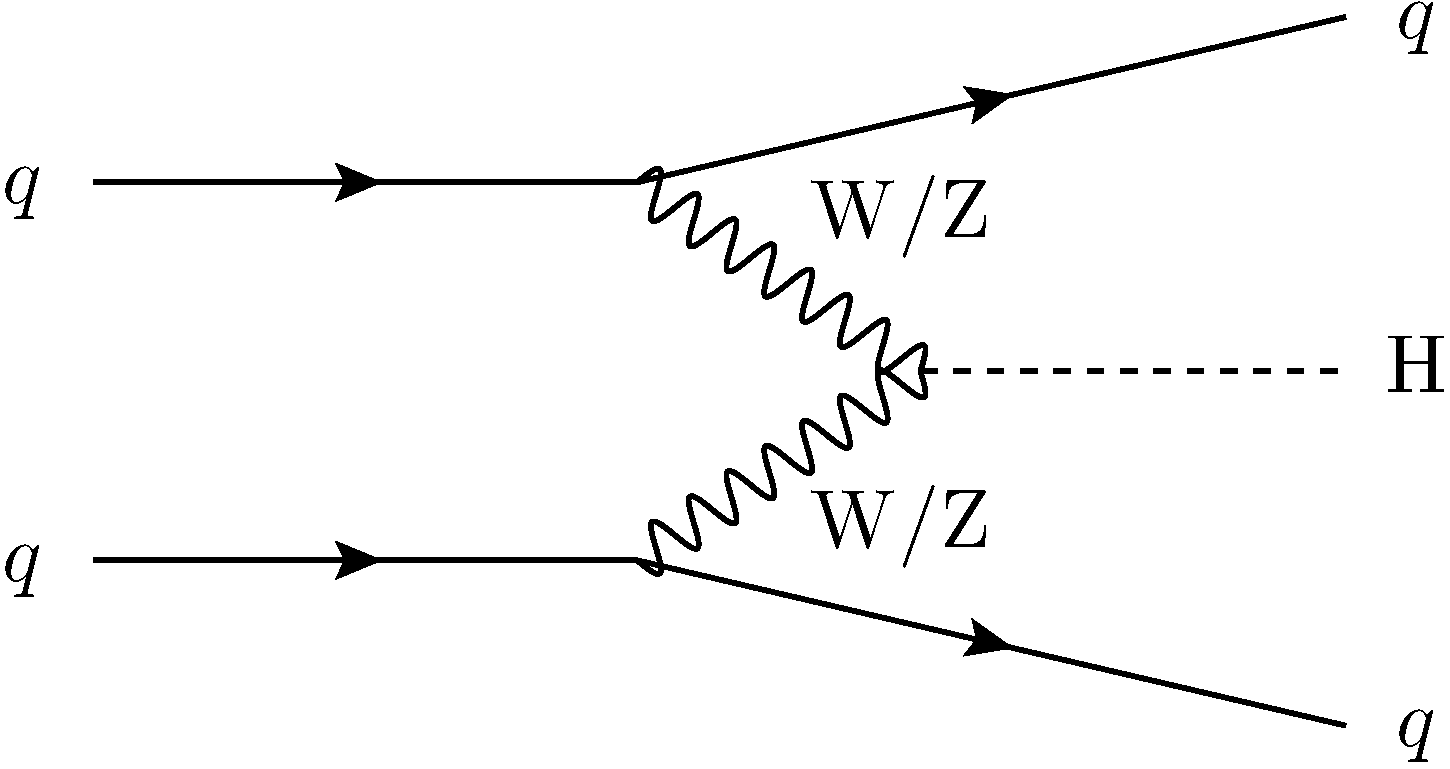
\includegraphics[width=0.5\textwidth]{./Theory/Figures/feynman_qqH.pdf}}~\\
\subfloat[W/Z associated production]{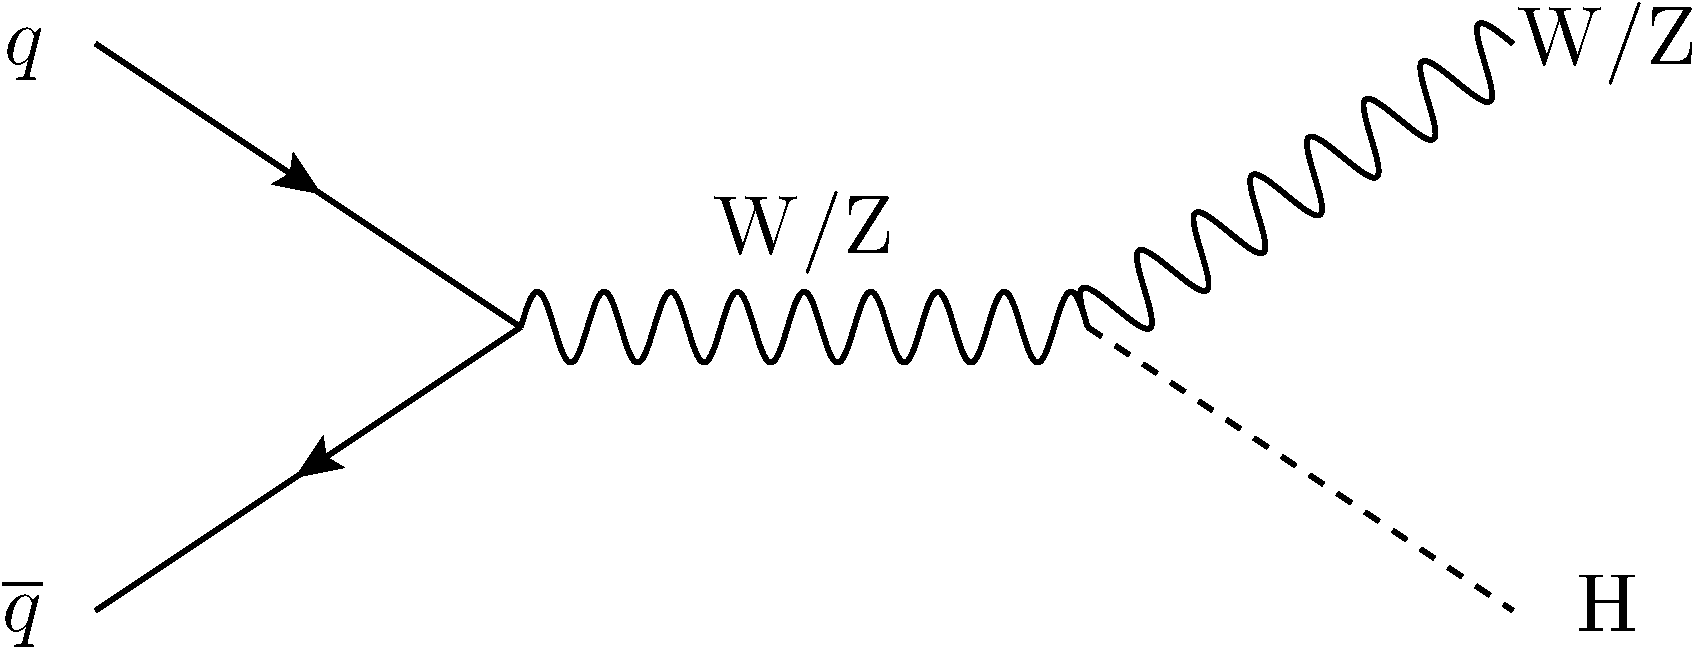
\includegraphics[width=0.5\textwidth]{./Theory/Figures/feynman_VH.pdf}}
\subfloat[\ttbar associated production]{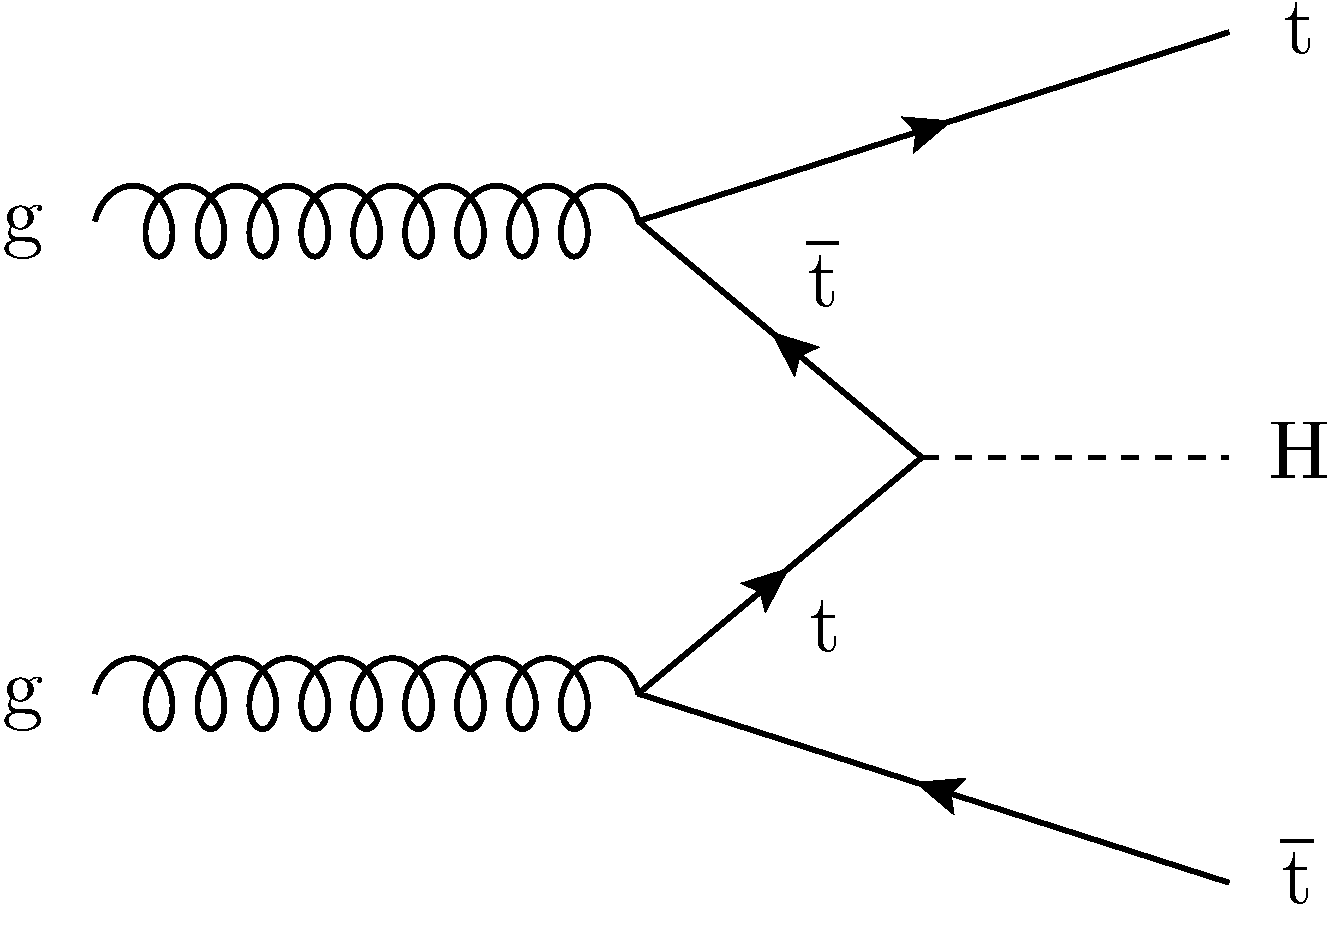
\includegraphics[width=0.5\textwidth]{./Theory/Figures/feynman_ttH.pdf}}
\end{center}
\caption{Feynman diagrams at tree level for the dominant Higgs boson production modes at
the \ac{LHC}.}
\label{fig:theory_smhprod}
\end{figure}

Figure \ref{fig:theory_smhprod} shows the dominant Higgs boson production modes
at the \ac{LHC}. From the production cross sections for each mode in figure
\ref{fig:theory_smhxsbr} we see that gluon fusion is by far dominant. The other modes
shown have smaller cross sections, but are of importance due to their topologies, with
additional leptons or jets in the final state. Tagging such topologies can reduce the size
of the \ac{SM} background.

\begin{figure}[h!]
\begin{center}
\subfloat[\ac{SM} H production cross sections]{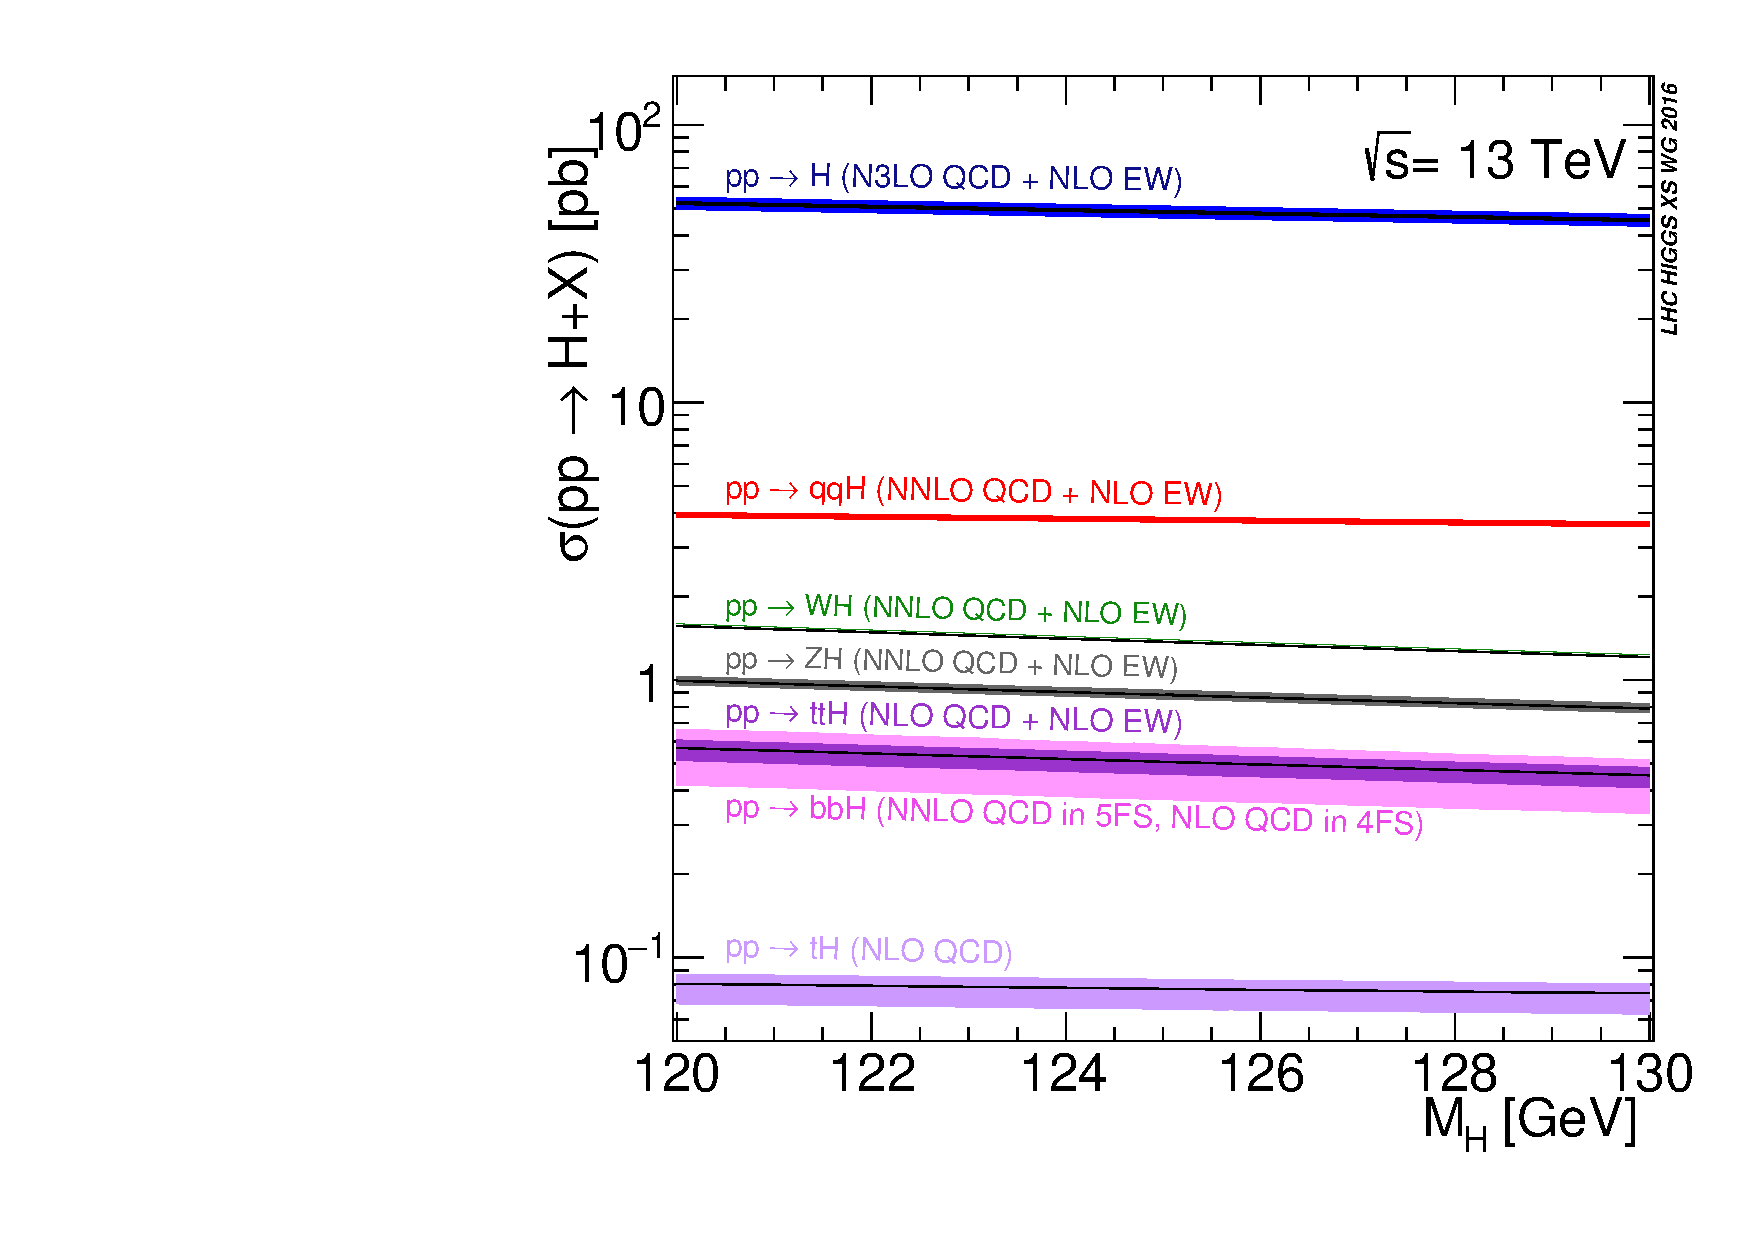
\includegraphics[width=0.5\textwidth]{./Theory/Figures/plot_13tev_H_sqrt.pdf}}
\subfloat[\ac{SM} H branching ratios]{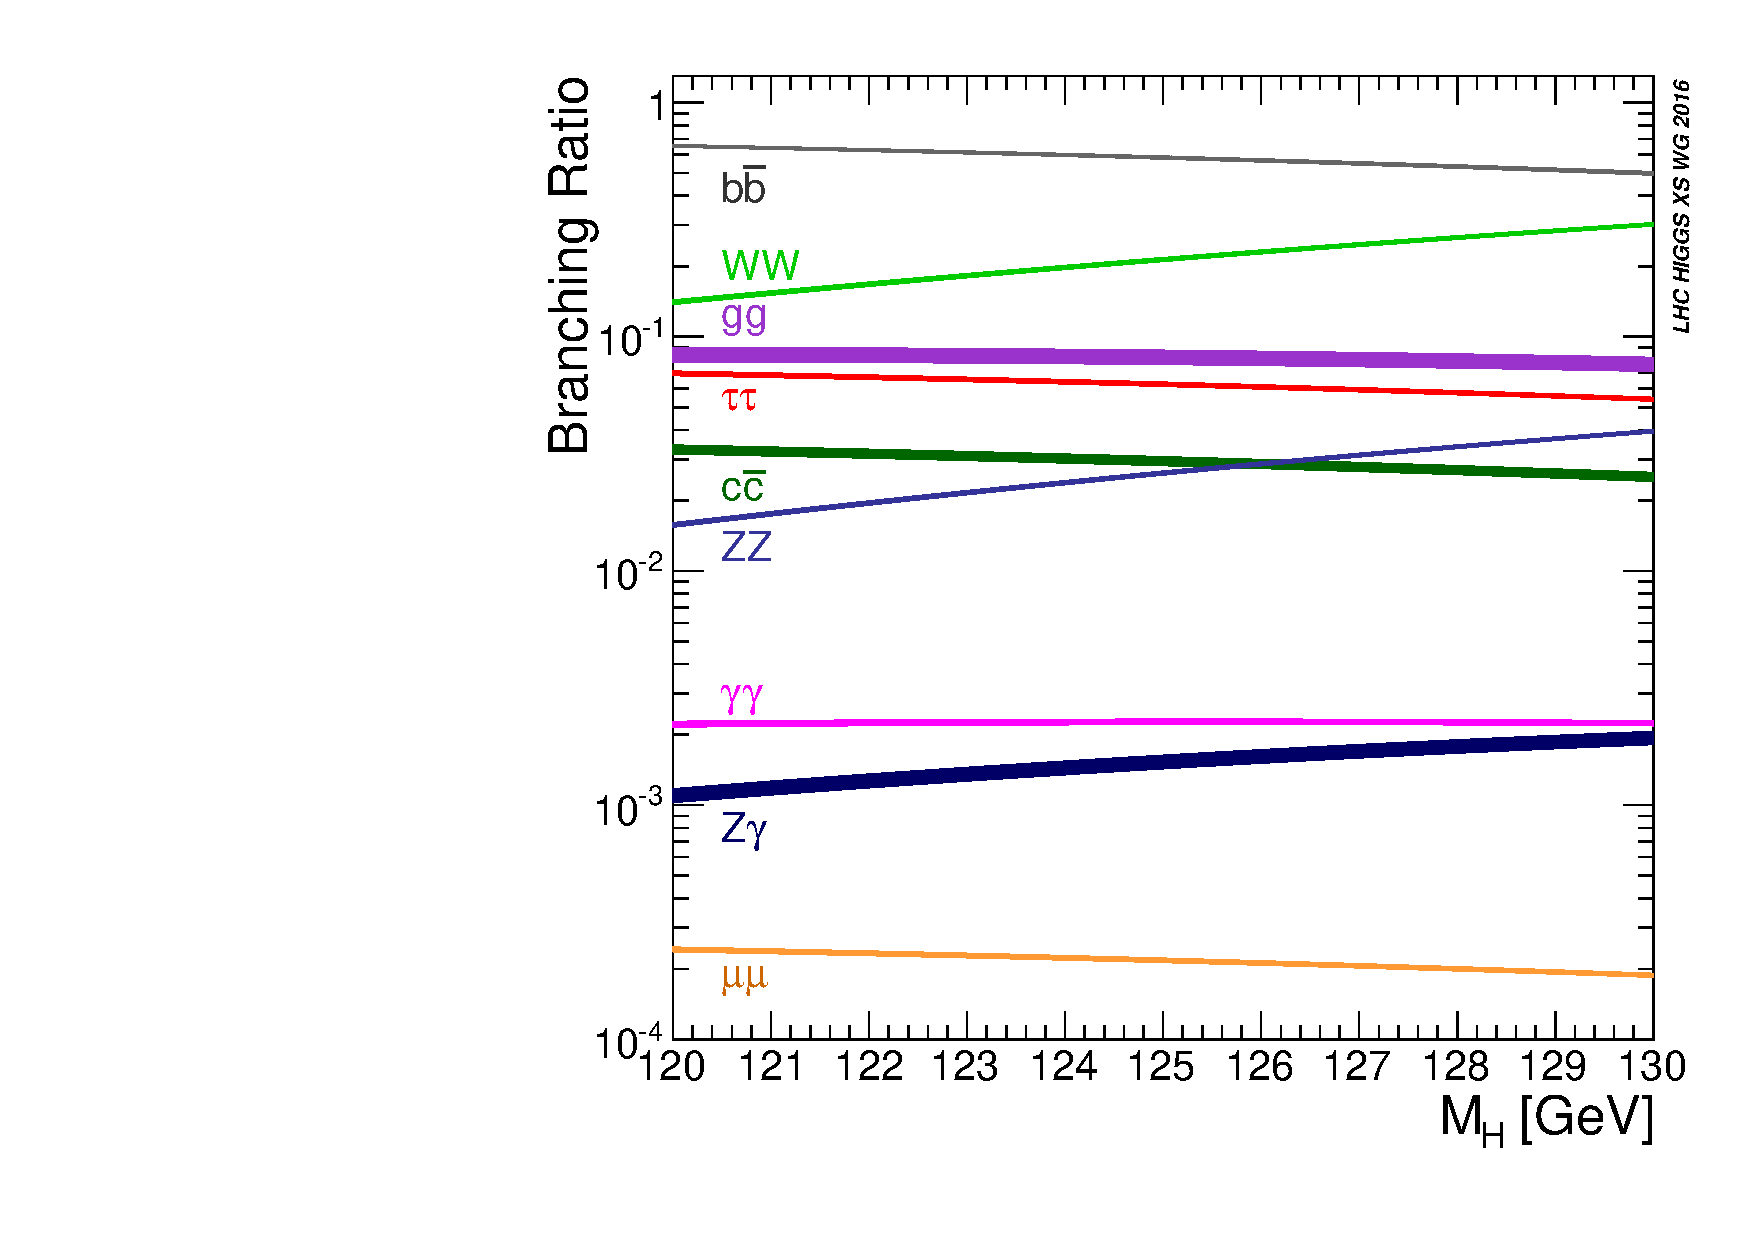
\includegraphics[width=0.5\textwidth]{./Theory/Figures/SMHiggsBRYR4-square.pdf}}
\end{center}
\caption{(a) standard model Higgs boson production cross sections at $\sqrt{s} = 13$ TeV and (b) standard model
Higgs boson branching ratios, for Higgs boson masses between 120 and 130 GeV \cite{YR4}.}
\label{fig:theory_smhxsbr}
\end{figure}

It is clear from the branching ratios of the \ac{SM} Higgs boson in figure \ref{fig:theory_smhxsbr}
that the two discovery channels $\PHiggslight \rightarrow \gamma\gamma$ and $\PHiggslight \rightarrow \PZ
PZ$ have smaller branching ratios than many other channels. These two channels are very sensitive
due to the small backgrounds and the excellent photon and lepton energy resolution the detectors provide.

During Run 2 of the LHC, standard model Higgs boson measurements, and searches for the 
standard model Higgs boson in decay channels not previously established, have 
already been performed. The decay in to $\gamma\gamma$ has been re-established \cite{CMSHgamgam2016,ATLASHgamgam2016},
as has the decay in to $ZZ\rightarrow 4\ell$ \cite{CMSHZZ2016,ATLASHZZ2016}. In addition, measurements
of $H\rightarrow WW$ are under way \cite{CMSHWW2016,ATLASHWW2016}. Establishment of the decay of 
$H\rightarrow b\bar{b}$ \cite{CMSVBFHbb2016,ATLASVHbb2016} and of $H\rightarrow \mu\mu$ \cite{ATLASHmm2016} 
is still to be achieved.
Finally, searches for ttH production, important to establish the top-Higgs coupling, have also been carried 
out \cite{CMSttH2016,CMSttHmultilep2016,ATLASttHbb2016,ATLASttHmultilep2016}. As the Run 2 dataset
keeps growing, more such measurements will be made to shed more light on the standard model Higgs boson.

\section{Beyond the standard model}
\label{sec:theory_BSM}
The \ac{SM} has been successfully tested to high accuraccy \cite{pdg-2014}. However,
some issues remain that cannot be addressed by the \ac{SM} alone \cite{griffiths}.
For example, it does not provide a candidate for dark matter. 
Additionally, the energy dependence of the running coupling constants
do not converge the GUT scale, and the force of gravity does not
appear in the \ac{SM}, no quantum theory can be formulated for it.

These issues aside, one of the most pressing issues regarding
the Higgs sector of the \ac{SM} is the hierarcy problem.
The \ac{SM}
is accepted to be an effective field theory that describes
the elementary particles and their interactions well up to an energy scale $\Lambda$.
This is the energy scale at which new physics must enter.
We know that $\Lambda \leq \mathcal{O}(10^{19})$, the Planck scale, as quantum 
gravitational effects start to become important in that region. $\Lambda$ enters
the corrections due to fermion and boson loops to the Higgs boson mass quadratically \cite{MSSM-carena-haber}:
\begin{equation}\label{eqn:mh_hierarchy}
m_{h_{\text{SM}}}^2  = (m_h^2)_0 + \mathcal{O}(\Lambda^2).
\end{equation}
Thus assuming that there is no new physics all the way up to
the Planck scale the observation \mh=125 GeV would only be compatible with $\Lambda$ of order $10^{19}$ GeV
if there was extreme fine-tuning of the bare Higgs boson mass $(m_h^2)_0$.

Many \acf{BSM} theories have been developed
that can to address the hierarchy problem and some of the other issues 
discussed. One of the most
popular of such theories is \acf{SUSY} \cite{SUSY-primer}, which postulates
that there is a symmetry between bosons and fermions. Every fermionic
\ac{SM} particle has a bosonic superpartner (named `s'+name of fermion, e.g.
sbottom, selectron,...), and every bosonic \ac{SM} particle
has a fermionic superpartner (named boson name + `ino', e.g. higgsino, Wino,...).

If this symmetry were unbroken the \ac{SUSY} particles must
have the same mass as their \ac{SM} partners. However, if that had 
been the case such particles would have been detected a long time ago. The 
only possibility is then that \ac{SUSY} is a broken symmetry and the superpartners
are heavier than their \ac{SM} equivalents. It is important to note
that the fermion and boson loops contribute to the Higgs boson
mass corrections with opposite sign, and so, if \ac{SUSY}
was an exact symmetry their contributions to the Higgs boson mass
would cancel. Due to 
symmetry breaking the contributions of \ac{SM} particles 
and their supersymmetric partners do not completely cancel. If
the \ac{SUSY} breaking scale, where new particles should
be found, is much larger than a few TeV further fine-tuning of 
the bare Higgs boson mass would be required \cite{MSSM-carena-haber,SUSY-primer}.
Apart from solving the hierarchy problem, \ac{SUSY} addresses some
of the other aforementioned issues. The lightest \ac{SUSY} particle
would be a candidate for dark matter if it were stable \cite{SUSY-primer}. On top of that
assuming \ac{SUSY} means the electroweak and strong coupling
constants intersect at a common energy scale of $\mathcal{O}(10^{16} \text{ GeV })$ \cite{GUT-LEP}. 

The simplest supersymmetric extension of the \ac{SM}, the \ac{MSSM} \cite{SUSY-primer}, only adds the minimum
number of particles and fields required to formulate a supersymmetric theory.
%And conserves R-parity, see section 6.2 of the SUSY primer


\subsection{The Higgs sector of the \ac{MSSM}}
\label{sec:theory_MSSM_H}
At least two Higgs doublets are required in the
Higgs sector of the \ac{MSSM} due to the supersymmetric
background of the theory \cite{MSSM-carena-haber}. Two complex Higgs doublets are added,
\begin{equation}\label{eqn:mssm_higgsdoublets}
\phi_d = \begin{pmatrix} \phi_d^0 \\
\phi_d^- \end{pmatrix} \text{ and } \phi_u = \begin{pmatrix} \phi_u^+ \\
\phi_u^0 \end{pmatrix}
\end{equation}
Note that $\phi_d^0$ couples exclusively to down-type fermions, and $\phi_u^0$ couples
exclusively to up-type fermions.
This leads to potential terms in the MSSM Lagrangian of the form:
\begin{equation}\label{eqn:mssm_lagrangian_potential}
V = \mu(\phi_u^+\phi_d^- - \phi_u^0\phi_d^0),
\end{equation}
with $\mu$ a mass parameter, equivalent to the \ac{SM} Higgs mass parameter.
This provides electroweak symmetry breaking as in the \ac{SM} case and
minimising this potential gives,
\begin{equation}\label{eqn:mssm_minimpot}
\langle 0|\phi_d| 0 \rangle = \begin{pmatrix}v_d\\
0 \end{pmatrix} \text{ and} \langle 0 |\phi_d|\rangle 0 = \begin{pmatrix} 0\\
v_u \end{pmatrix}
\end{equation}
Using this we define
\begin{equation}\label{eqn:tanb_def}
\tan{\beta} \equiv \frac{v_u}{v_d}
\end{equation}
Of the eight degrees of freedom due to the introduction of two complex
doublets, three become longitudinal states of the $\PW^{\pm}$ and \PZ bosons.
The remaining 5 degrees of freedom lead to five physical Higgs bosons, a charged
Higgs boson pair $\PHiggs^{\pm}$, the neutral pseudoscalar \PHiggsps
and the neutral scalars h and H. These are defined in terms
of \tanb~and a mixing angle $\alpha$ which arises from diagonalising
the neutral scalar Higgs squared-mass matrix, see equation \ref{eqn:treelevel_mass}. The five bosons become:
\begin{align}\label{eqn:MSSMHiggsMixing}
&\PHiggs^+ = \phi_u^+\cos{\beta} + \phi_d^{-\dagger}\sin{\beta},\\
&\PHiggs^- = \phi_u^{+\dagger}\cos{\beta} + \phi_d^{-}\sin{\beta},\\
&\PHiggsps = \sqrt{2}(\text{Im}\phi_d^0\sin{\beta} + \text{Im}\phi_u^0\cos{\beta}),\\
&\PHiggslight = -(\sqrt{2}\text{Re}\phi_d^0 - v_d)\sin{\alpha} + (\sqrt{s}\text{Re}\phi+u^0 -v_u)\cos{\alpha}\\
&\PHiggs = (\sqrt{2}\text{Re}\phi_d^0-v_d)\cos{\alpha}+(\sqrt{2}\text{Re}\phi_u^0-v_u)\sin{\alpha}
\end{align}
As the self-interactions of the Higgs fields are not independent parameters
but are functions of the electroweak gauge coupling constants, at tree
level the MSSM Higgs sector parameters are determined by two free parameters, \tanb~and
one of the Higgs boson masses, conventionally chosen as \mA.
Using this the masses of the five Higgs states are found as:
\begin{equation}\label{mssm_chargedhigss_mass}
m_{\PHiggs^{\pm}}^2 = m_{\PHiggsps}^2+m_{\PW}^2,
\end{equation}
while the neutral scalar \PHiggslight and \PHiggs are eigenstates of the tree-level
squared-mass matrix:
\begin{equation}\label{eqn:treelevel_mass}
\mathcal{M}_{\text{tree}}^2 = \begin{pmatrix} 
m_{A}^2\sin{\beta}^2 + m_{Z}^2\cos{\beta}^2 & -(m_{A}^2+m_{Z}^2)\sin{\beta}\cos{\beta}\\
-(m_{A}^2+m_{Z}^2)\sin{\beta}\cos{\beta} & m_{A}^2\cos{\beta}^2+m_{Z}^2\sin{\beta}^2 \end{pmatrix}.
\end{equation}
This leads to the masses of \PHiggslight and \PHiggs as eigenvalue of $\mathcal{M}_{\text{tree}}^2$,
\begin{equation}\label{eqn:scalarmass}
m_{\PHiggs,\PHiggslight}^2 = \frac{1}{2}(m_{A}^2+m_{Z}^2 \pm \sqrt{(m_A^2+m_Z^2)^2-4m_Z^2m_A^2\cos{2\beta}^2}).
\end{equation}
A consequence of this is a tree-level upper bound to the mass of the light Higgs
boson,
\begin{equation}\label{eqn:mh_upper}
m_{h} \leq m_{Z},
\end{equation}
and a constraing on $\alpha$,
\begin{equation}\label{eqn:alpha_constraint}
\cos{(\beta-\alpha)}^2 = \frac{m_h^2(m_Z^2-m_h^2)}{m_A^2(m_H^2-m_h^2)}.
\end{equation}

The constraint on $m_h$ being less than the mass of the Z boson, 91.2 GeV, seems 
problematic at first, as we know there is a Higgs state with a mass of 125 GeV. However,
the tree-level masses and couplings of the Higgs bosons in the MSSM can be
significantly altered by radiative corrections. The dominant effect is from
incomplete cancellation of the stop- and top-loop corrections, which
do not completely cancel as SUSY is a broken symmetry.

The tree-level couplings of the neutral Higgs bosons to bosons and fermions 
are modified with respect to the \ac{SM} couplings, by factors
described in table \ref{tab:mssm_couplings} \cite{YR4}.

\begin{table}[htp]
\label{tab:mssm_couplings}
\begin{center}
\caption{Tree-level couplings in the MSSM, as multiplicative factors with
respect to the \ac{SM} couplings}
\begin{tabular}{p{2cm}p{4cm}p{4cm}p{4cm}}
\toprule
Particle & Coupling to bosons & Coupling to up-type quarks & Coupling to down-type quarks and leptons \\
\midrule
\PHiggsps & 0 & $\cot{\beta}$ & $ \tan{\beta}$\\
\PHiggs & $\cos{\beta-\alpha}$ & $\frac{\sin{\alpha}}{\sin{\beta}}$ & $\frac{\cos{\alpha}}{\cos{\beta}}$\\
\PHiggslight & $\sin{\beta-\alpha}$ & $\frac{\cos{\alpha}}{\sin{\beta}}$ & $-\frac{\sin{\alpha}}{\cos{\beta}}$\\
\bottomrule
\end{tabular}
\label{tab:mssm_couplings}
\end{center}
\end{table}

In the \textit{decoupling limit}, when \mA$>>m_{Z}$ and $\cos{(\beta-\alpha)}$ tends
to 0, the mixing
angle $\alpha \approx \beta - \pi/2$. This reduces the couplings in table
\ref{tab:mssm_couplings} to the \ac{SM} couplings for the \PHiggslight boson, 
with negligible couplings to bosons for the two remaining neutral
Higgs bosons, couplings to down-type quarks and leptons enhanced by a factor \tanb,
and couplings to up-type quarks enhanced by a factor $\frac{1}{\tan{\beta}}$. This motivates
the choice of decay into $\Pgt\Pgt$ as search channel for the neutral Higgs bosons in the MSSM.
Figure \ref{fig:mssm_brtautau} shows the branching ratios of the \PHiggs boson 
in the $m_{h}^{\text{mod+}}$ scenario
which will be discussed in more detail in section \ref{sec:theory_BSM_models_mhmodp}. 
The branching ratio into di-$\Pgt$ pairs is large for \tanb=30. The branching ratios 
into $\Pgt\Pgt$ of \PHiggsps are of similar size.
%Using trigon identities: cos alpha/cos beta = cos (beta-pi/2)/cos beta = cosbeta*cospi/2 + sin(beta)*sin(pi/2) over cos beta = sin beta /cos beta = tan beta
%sin alpha = sin (beta-pi/2) = sinbeta cos pi/2 - cosbetasinpi/2 = -cosbeta 
%such that -sinalpha/cosbeta = 1
%cos alpha/sin beta = sin beta/sin beta = 1
%sin beta-alpha = sin pi/2 = 1
%cos beta-alpha = cos pi/2 = 0
%sin alpha/sin beta = -cos beta/sin beta=-1/tan(beta)

\begin{figure}[h!]
\begin{center}
\subfloat[\tanb=5]{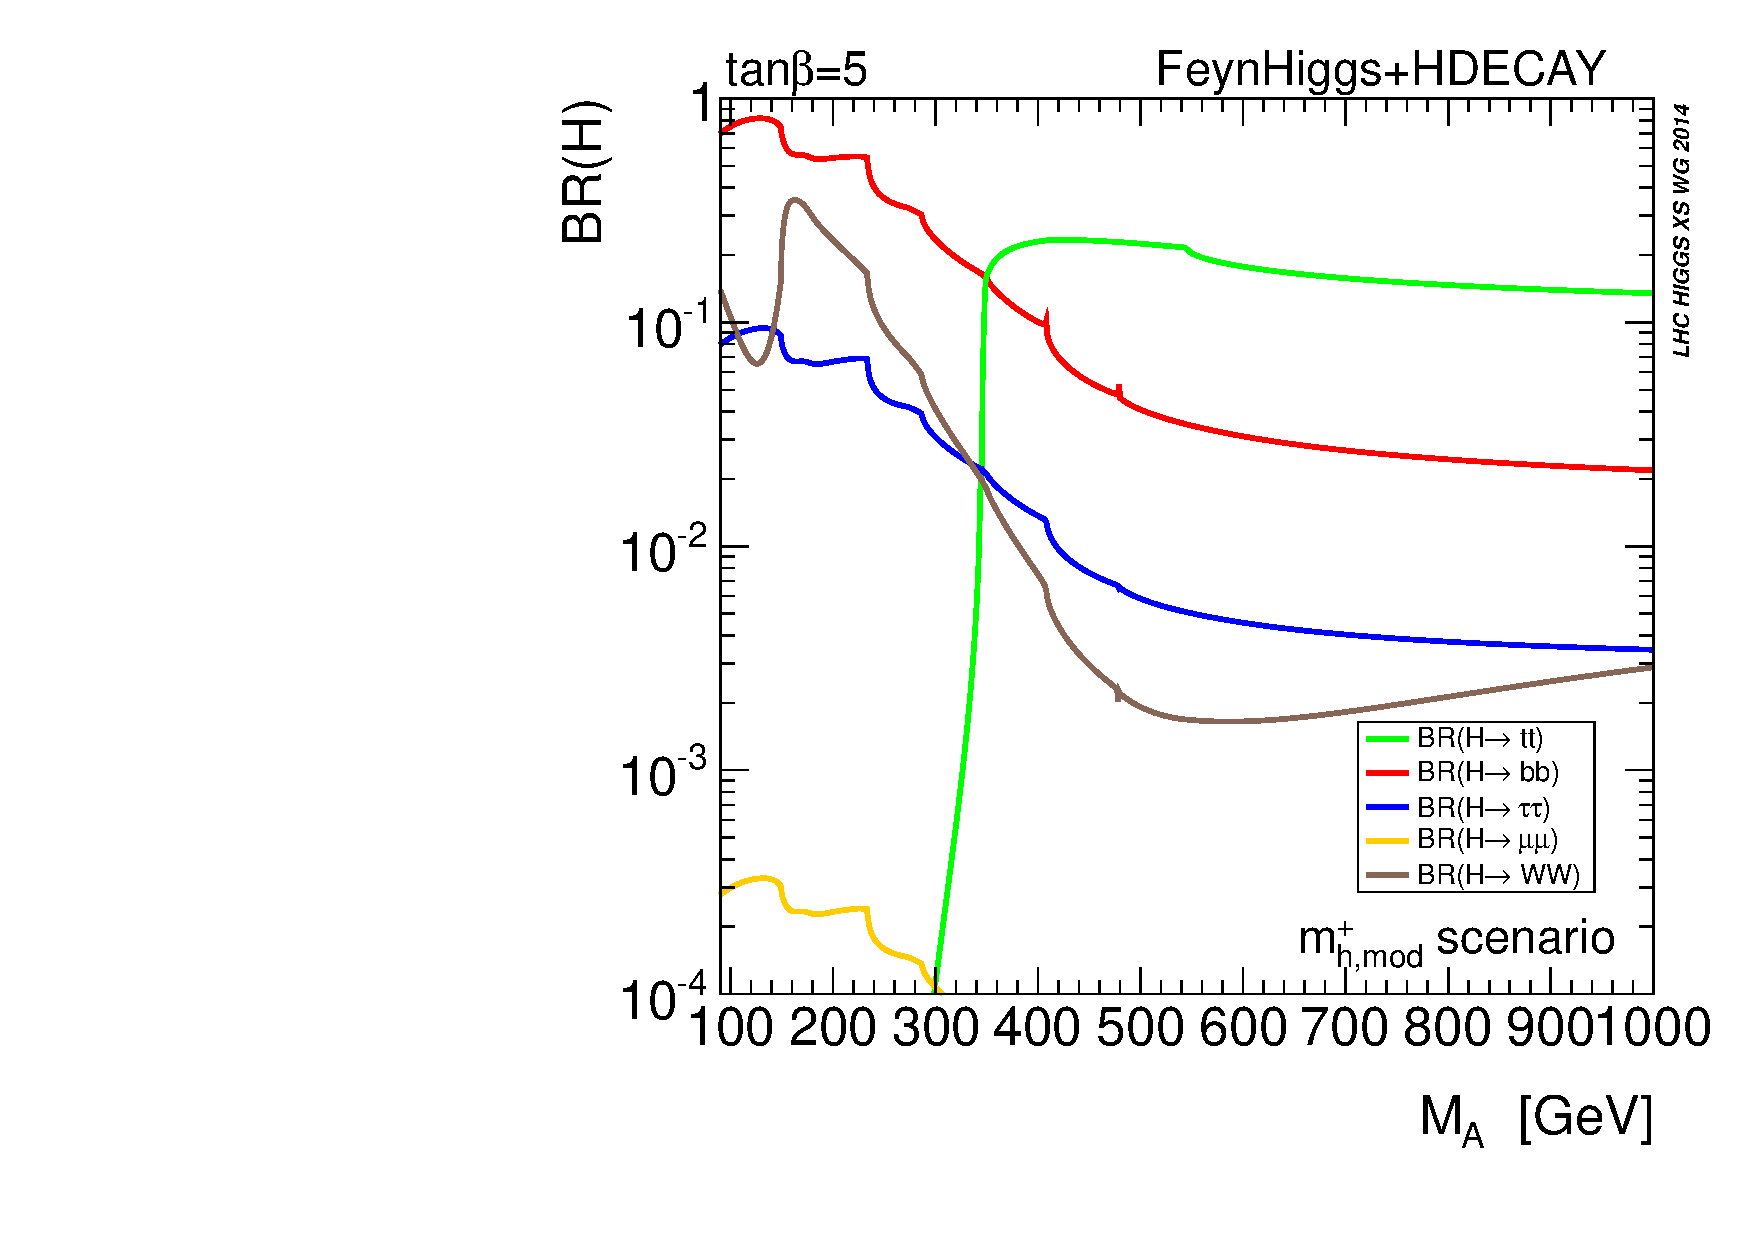
\includegraphics[width=0.5\textwidth]{./Theory/Figures/YR4HXS_BRSummary_H_mhmodp_tanbeta5_FeynHiggs_HDecay.pdf}}
\subfloat[\tanb=30]{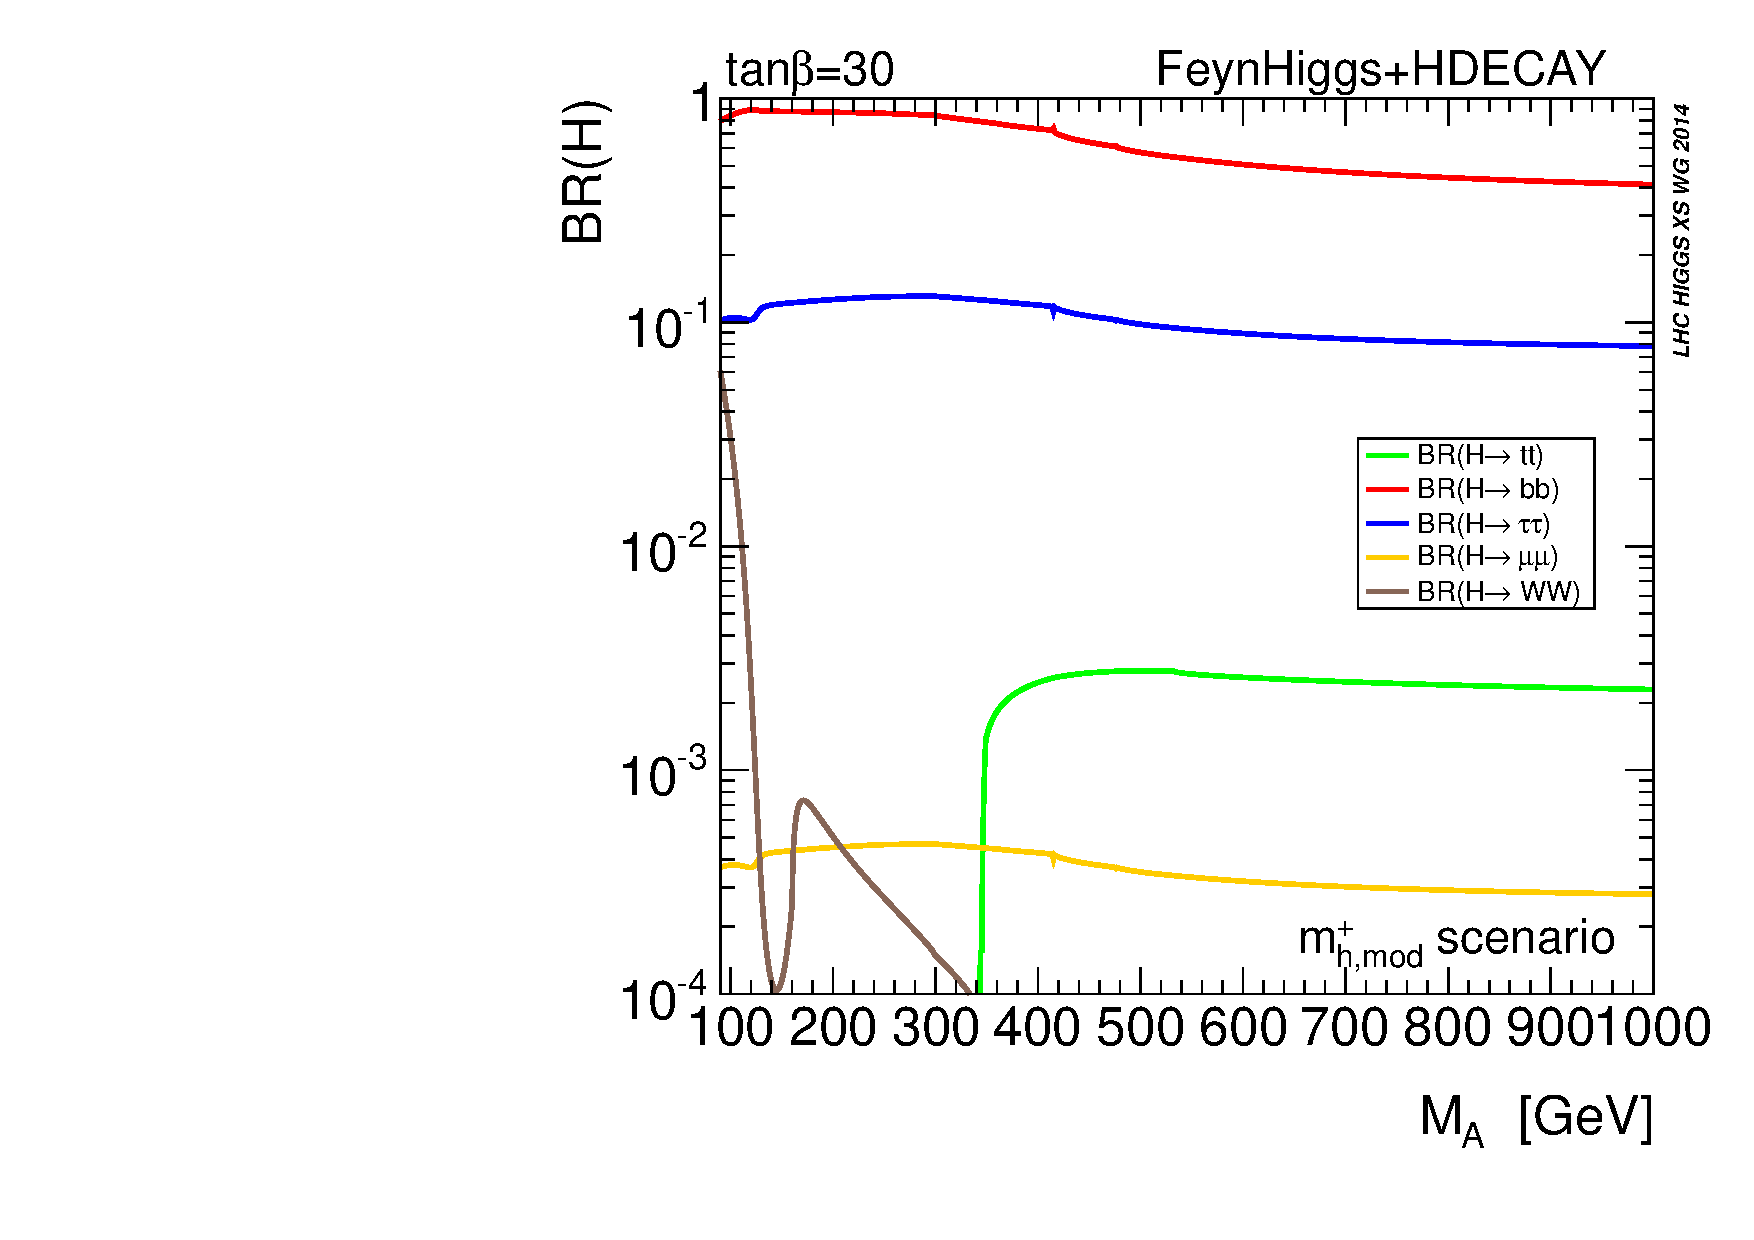
\includegraphics[width=0.5\textwidth]{./Theory/Figures/YR4HXS_BRSummary_H_mhmodp_tanbeta30_FeynHiggs_HDecay.pdf}}
\end{center}
\caption{Branching ratios of the \PHiggs boson in the $m_{h}^{\text{mod+}}$ scenario,
at (a) \tanb=5~and (b) \tanb=30. The branching ratio into \Pgt\Pgt (blue), $b\bar{b}$ (red) 
and \Pgm\Pgm (yellow) is enhanced at high \tanb, while the branching ratio into 
WW (grey) and \ttbar (green) is reduced \cite{MSSM-xswg-twiki}.}
\label{fig:mssm_brtautau}
\end{figure}

The dominant neutral MSSM Higgs boson production processes at hadron colliders
are slightly different from the \ac{SM} Higgs boson production processes. 
Because the pseudoscalar A does not couple to the
vector bosons, and in the decoupling limit the coupling of \PHiggs to vector
bosons is suppressed with respect to the \ac{SM} expectation, VBF and PW/PZ associated
production do not constitute dominant production processes. Gluon fusion production is 
the dominant production mode at low \tanb, like in the \ac{SM}. An example tree-level Feynman diagram is given in figure \ref{fig:production_mssm}a. In gluon fusion production the Higgs boson
is produced via a quark loop. At low \tanb~values this loop is dominated by top quarks, while at 
high \tanb~the b-quark loop dominates. This is a result of the enhanced coupling to down-type fermions at high \tanb. Another consequence of these enhanced couplings to down-type fermions at high \tanb~is the dominance of b-associated production, where the Higgs boson is produced through
bottom quark fusion. The tree-level Feynman diagram for this process is shown in figure \ref{fig:production_mssm}b.

\begin{figure}[h!]
\begin{center}
\subfloat[gluon fusion production]{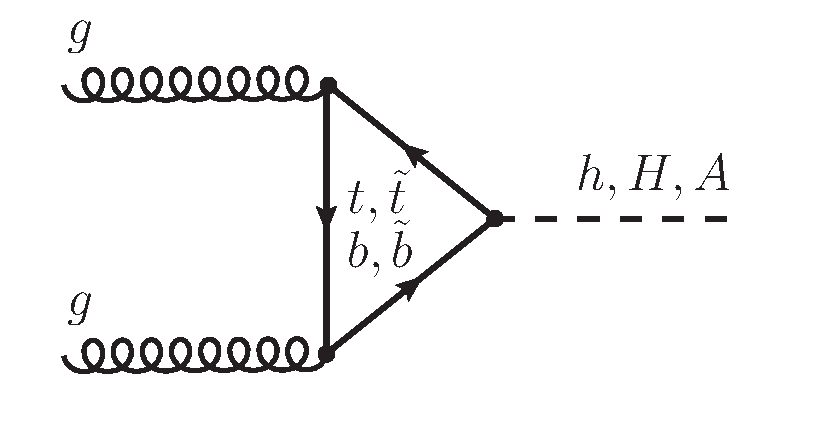
\includegraphics[width=0.5\textwidth]{./Theory/Figures/CMS-PAS-HIG-16-037_Figure_001-a.pdf}}
\subfloat[b-associated production]{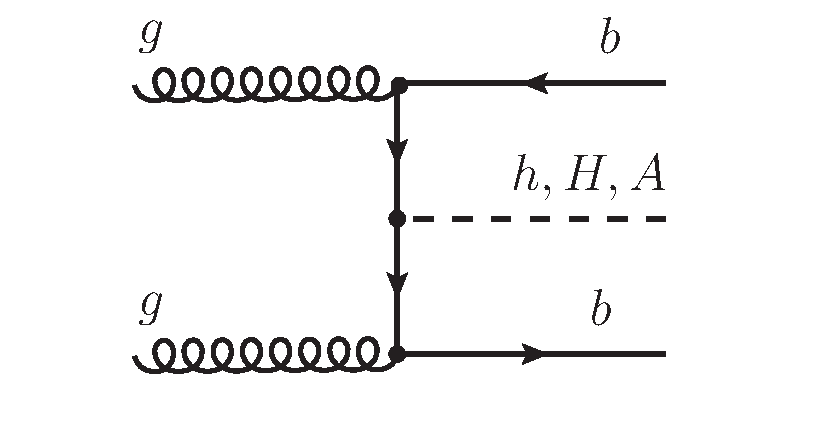
\includegraphics[width=0.5\textwidth]{./Theory/Figures/CMS-PAS-HIG-16-037_Figure_001-b.pdf}}
\end{center}
\caption{Tree-level Feynman diagrams of (a) gluon fusion production and (b) b-associated
production of neutral Higgs boson in the MSSM \cite{CMS-PAS-HIG-16-037}.}
\label{fig:production_mssm}
\end{figure}

\subsection{\acl{2HDM}s}
\label{sec:theory_2HDM}
A different approach, also leading to an extended Higgs sector with
respect to the \ac{SM} case, is found in the \ac{2HDM} \cite{2HDM-I,2HDM-II}.
As the name suggests \ac{2HDM}s are a generic class of models in which
there is not one, but two Higgs doublets. The addition of a second
Higgs doublet can also motivated by \ac{SUSY}, but also by axion models.
An important point to note is that despite the presence of a second 
Higgs doublet, there are no explicit \ac{SUSY} particles in the \ac{2HDM}.
There are many different types of \ac{2HDM}, all distinguished by the couplings
of the different Higgs bosons to bosons and fermions. The 
most general potential for a CP-conserving 2HDM has 9 free parameters,
taken as \tanb, the mixing angle $\alpha$, already discussed in 
the context of the \ac{MSSM}, the masses of the five Higgs bosons,
and quartic couplings appearing in the potential. The most studied of the
\ac{2HDM}s, the type-II \ac{2HDM}, has a structure very similar to 
the MSSM Higgs sector. The tree-level couplings of the neutral Higgs bosons to 
vector bosons and fermions are the same as the tree-level \ac{MSSM} couplings 
from table \ref{tab:mssm_couplings}. %The decay \AtoZh is also possible,
%the \AtoZh~coupling is proportional to $\cos{(\beta-\alpha)}, like the \Htohh~coupling.

The behaviour of the \ac{2HDM} couplings in the \textit{alignment} limit,
where $\cos{(\beta-\alpha)} = 0$, differs from that of the \ac{MSSM} couplings.
In particular, in the alignment limit the decays \AtoZh~and \Htohh vanish
in the \ac{2HDM}. This is due to the fact that the coupling is 
proportional to $\cos{(\beta-\alpha)}$ and there are no radiative corrections
to make the branching ratio nonzero.

The inclusive $\sigma\times$branching ratios for production of a \PHiggs boson 
and decays into various states is shown in figure \ref{fig:2hdm_Hxsbr}a for an 
example of a type-II \ac{2HDM}, at two \tanb points. Figure \ref{fig:2hdm_Hxsbr}b 
shows the inclusive $\sigma\times$branching ratios for production and decay
of a \PHiggsps boson in the same type-II \ac{2HDM} example, at two \tanb~points. At
low \tanb~the $\sigma\times$branching ratio for \Htohh production and decay and \AtoZh production
and decay are enhanced for $250\leq m_{\PHiggs}\leq 350$ GeV and $220 \leq m_{\PHiggsps} \leq 350$ GeV, respectively.

\begin{figure}[h!]
\begin{center}
\subfloat[\PHiggs]{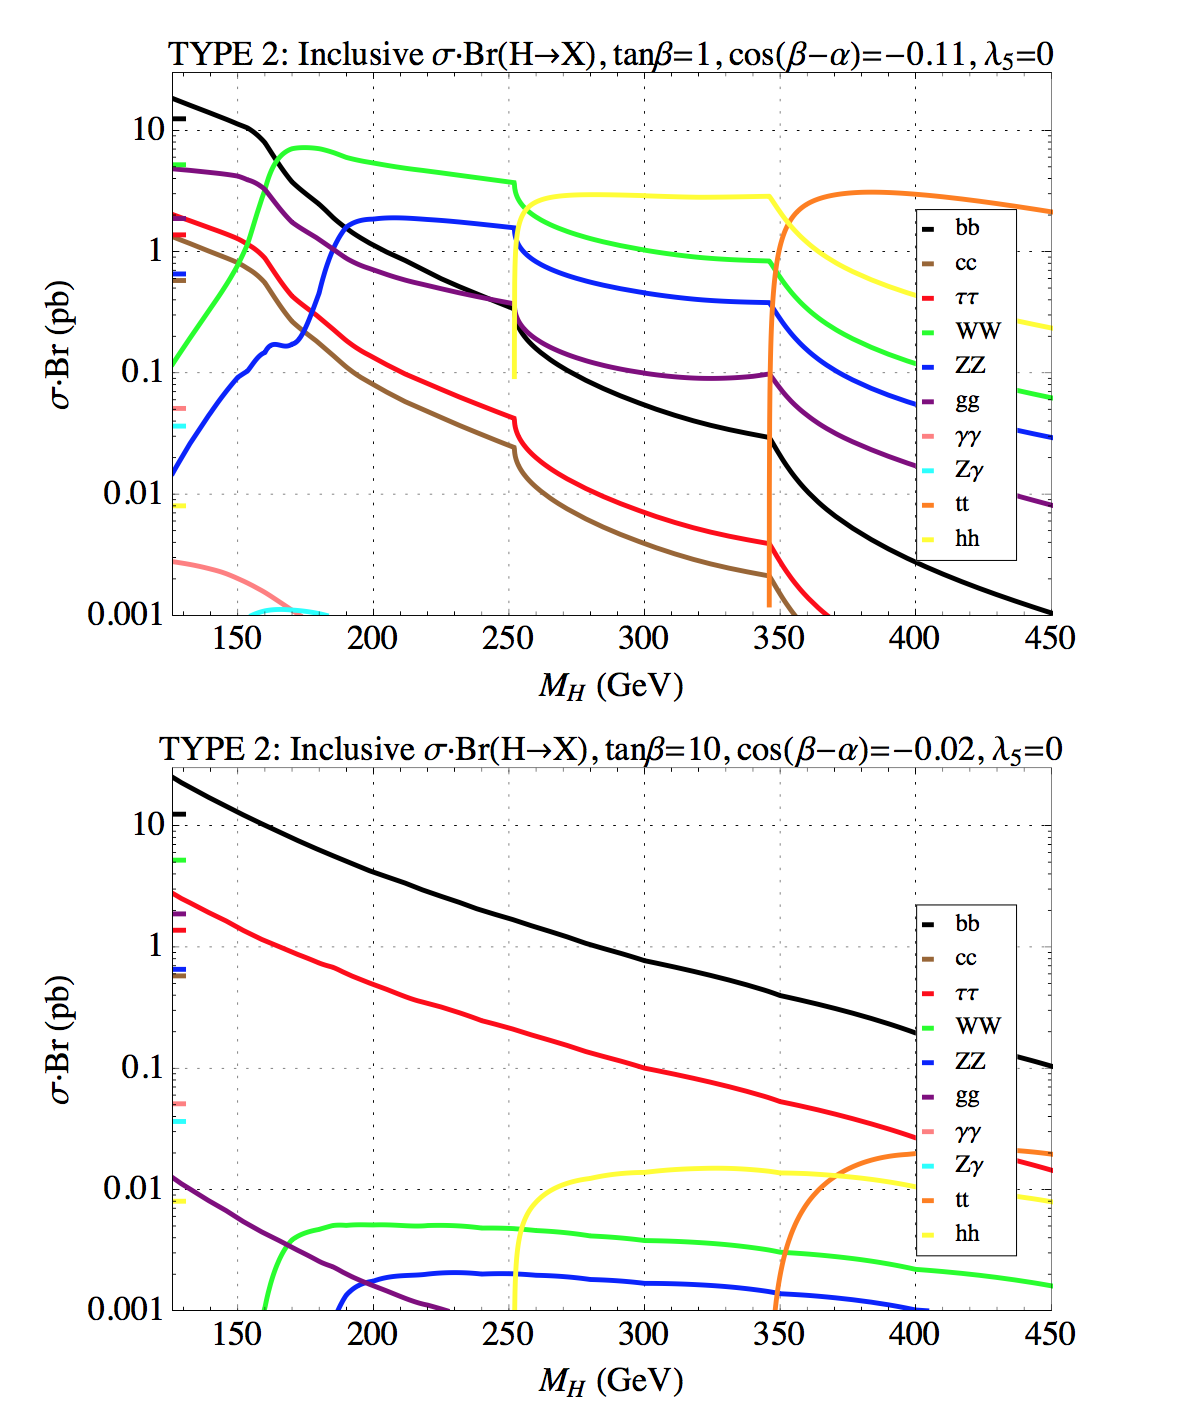
\includegraphics[width=0.5\textwidth]{./Theory/Figures/typeII2HDMxsbr.png}}
\subfloat[\PHiggsps]{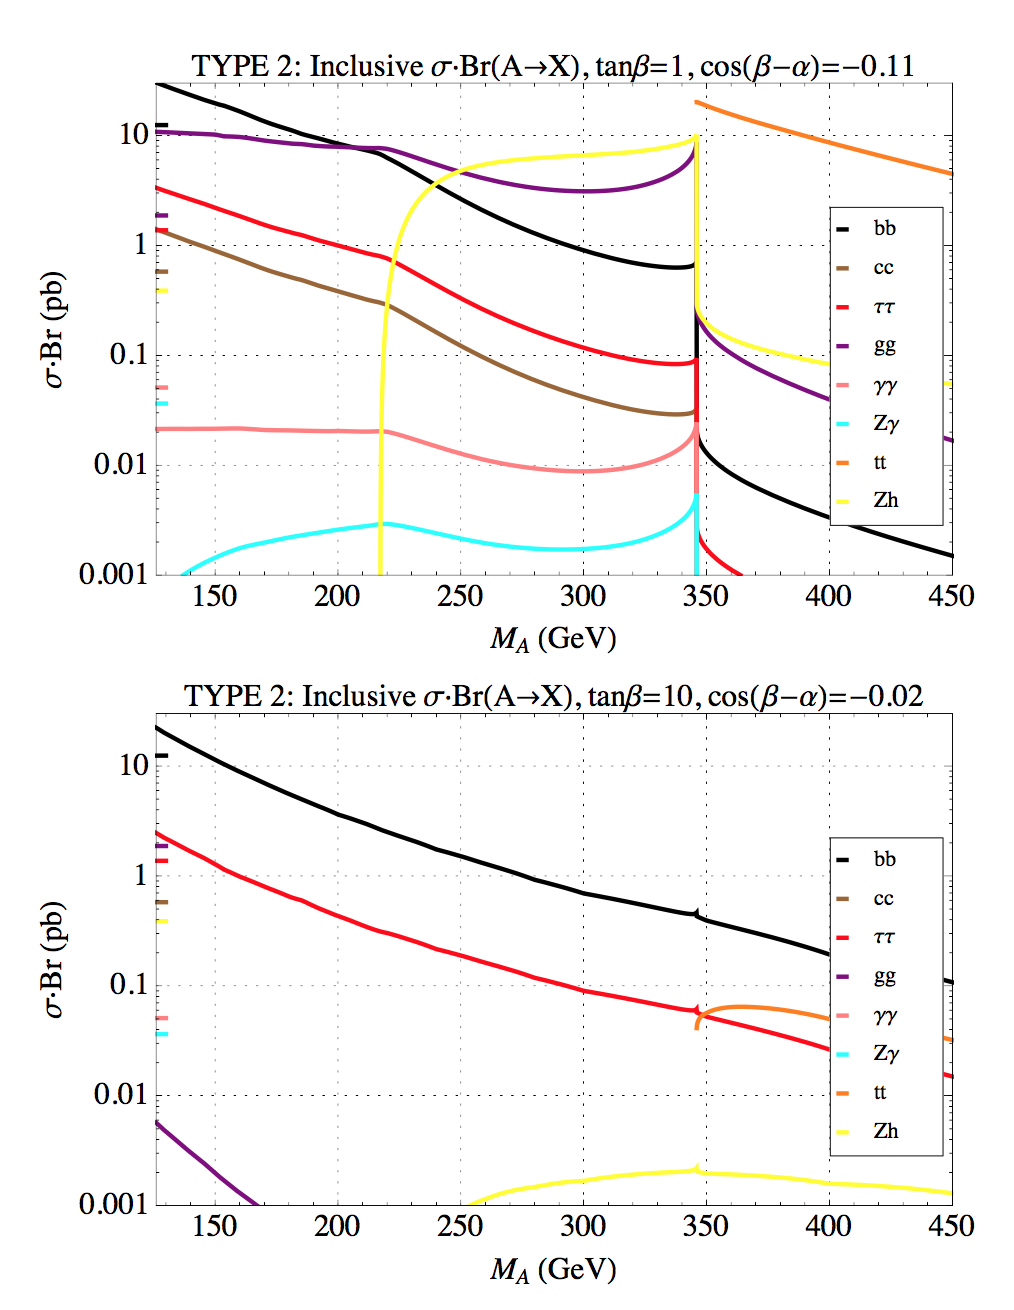
\includegraphics[width=0.5\textwidth]{./Theory/Figures/typeII2HDMxsbrA.png}}
\end{center}
\caption{Inclusive production cross--section times branching ratio for an example
of a type-II \ac{2HDM}, for (a) the \PHiggs boson and (b) the \PHiggsps boson. The
top figures use \tanb=1 and $\cos{(\beta-\alpha)}=-0.11$, the bottom
figures are made for \tanb=10 and $\cos{(\beta-\alpha)}=-0.02$. At low \tanb~the \Htohh and
\AtoZh decays are enhanced for masses up to 350 GeV \cite{2HDM-II}.}
\label{fig:2hdm_Hxsbr}
\end{figure}


\section{MSSM benchmark scenarios}
\label{sec:theory_BSM_models}
Because the MSSM contains a large number of
SUSY-breaking parameters that affect the Higgs
sector, it us usual to define benchmark scenarios 
in which the only free parameters are \mA~and \tanb.
In these scenarios the SUSY parameters entering in 
the radiative corrections are fixed to define the scenario.

The parameters that need to be fixed in the benchmark scenarios are:
\begin{itemize}
\item The mass of the third generation squarks, given by $M_{\text{SUSY}}$.
\item The higgsino mass parameter, $\mu$.
\item The mass of the stau, the third generation sleptons, $M_{\tilde{\ell_3}}$.
\item The mass of the gluino, $M_{\tilde{g}}$.
\item The U(1) gaugino mass parameter, $M_1$.
\item The SU(2) gaugino mass parameter, $M_2$.
\item The trilinear couplings of the stops, sbottoms and staus to the Higgs: $A_t$, $A_b$ and $A_{\Pgt}$.
\item The stop, sbottom and stau mixing parameters, $X_t$, $X_b$ and $X_{\Pgt}$.
\end{itemize}

Some of these parameters can be expressed in terms of relations to other parameters. 
$X_t$, $X_b$ and $X_{\Pgt}$ can be expressed as,
\begin{equation}\label{eqn:trilinear_couplings}
\begin{split}
&X_t = A_t-\mu\cot{\beta},\\
&X_b = A_b-\mu\tan{\beta},\\
&X_{\Pgt} = A_{\Pgt} - \mu\tan{\beta}.
\end{split}
\end{equation}
In addition, $M_1$ is fixed via the unification
relation,
\begin{equation}
M_1 = \frac{5}{3}M_s\tan{\theta_w}^2,
\end{equation}
where $\theta_w$ is defined by $\cos{\theta_w} = \frac{m_W}{m_Z}$.

Some additional parameters which have only a
small effect on the MSSM Higgs boson sector are alos considered.
Because their effect is so small they are
fixed in all benchmark scenarios at values compatible with 
exclusion limits from direct searches:
\begin{itemize}
\item Masses of the first and second generation squarks, $M_{\tilde{q}_{1,2}} = 1.5$ TeV.
\item Masses of the first and second generation sleptons, $M_{\tilde{\ell}_{1,2}} = 500$ GeV.
\item Trilinear couplings of first and second generation squarks and sleptons, $A_f=0$.
\end{itemize}

After the discovery of the 125 GeV Higgs boson the MSSM benchmark
scenarios need to accommodate this particle, which means only the 
scenarios which contain a light Higgs boson with a mass of around 125 GeV
are still accessible.

% in the mmax scenario the benchmark values have been chosen h
%such that the mass of the light CP-even Higgs boson is maximized for fixed tanβ and large
%MA (the scale of the soft SUSY-breaking masses in the stop and sbottom sectors, which
%sets the mass scale for the corresponding supersymmetric particles, has been fixed to 1 TeV
%in this scenario). This scenario is useful to obtain conservative bounds on tanβ for fixed
%values of the top-quark mass 

\subsection{The $m_{h}^{\text{mod+}}$ scenario}
\label{sec:theory_BSM_models_mhmodp}
The $m_{h}^{\text{mod+}}$ scenario \cite{MSSM-benchmark-scenarios}
is a modification of the $m_h^{\text{max}}$ scenario \cite{MSSM-mhmax}. This scenario, which
was used for interpretations of MSSM Higgs boson searches at LEP, allows
the mass of the light Higgs boson to reach the highest a-priori expected 
value of around 135 GeV for high \mA. There is only a small area of the \mA-\tanb~plane
in this scenario where the mass of the light Higgs boson is compatible with the
observed 125 GeV state. The modifications to the parameters of the $m_{h}^{\text{max}}$ 
scenario address this issue. In the $m_{h}^{\text{mod+}}$ scenario $M_{\text{SUSY}}$ is chosen
to be 1 TeV. The stop mixing parameter is positive, $X_t= 1.5 M_{\text{SUSY}}$.
%This gives better agreement with muon g-2 results while the mhmod- scenario
%negative stop mixing (-1.9 M_SUSY) results in better agreements with B(b->sgamma) 
%meausrements 
The remaining parameters are set as $\mu=200$ GeV, $m_{\tilde{g}} = 1.5$ TeV,
$m_{\tilde{\ell}_3} = 1$ TeV, and $A_b=A_t=A_{\Pgt}$. Figure \ref{fig:mhmodp_mh}
shows the mass of the light Higgs boson in the $m_{h}^{\text{mod+}}$ scenario, showing
that its mass is compatible with 125 GeV over a large part of the parameter space.
\begin{figure}[h!]
\begin{center}
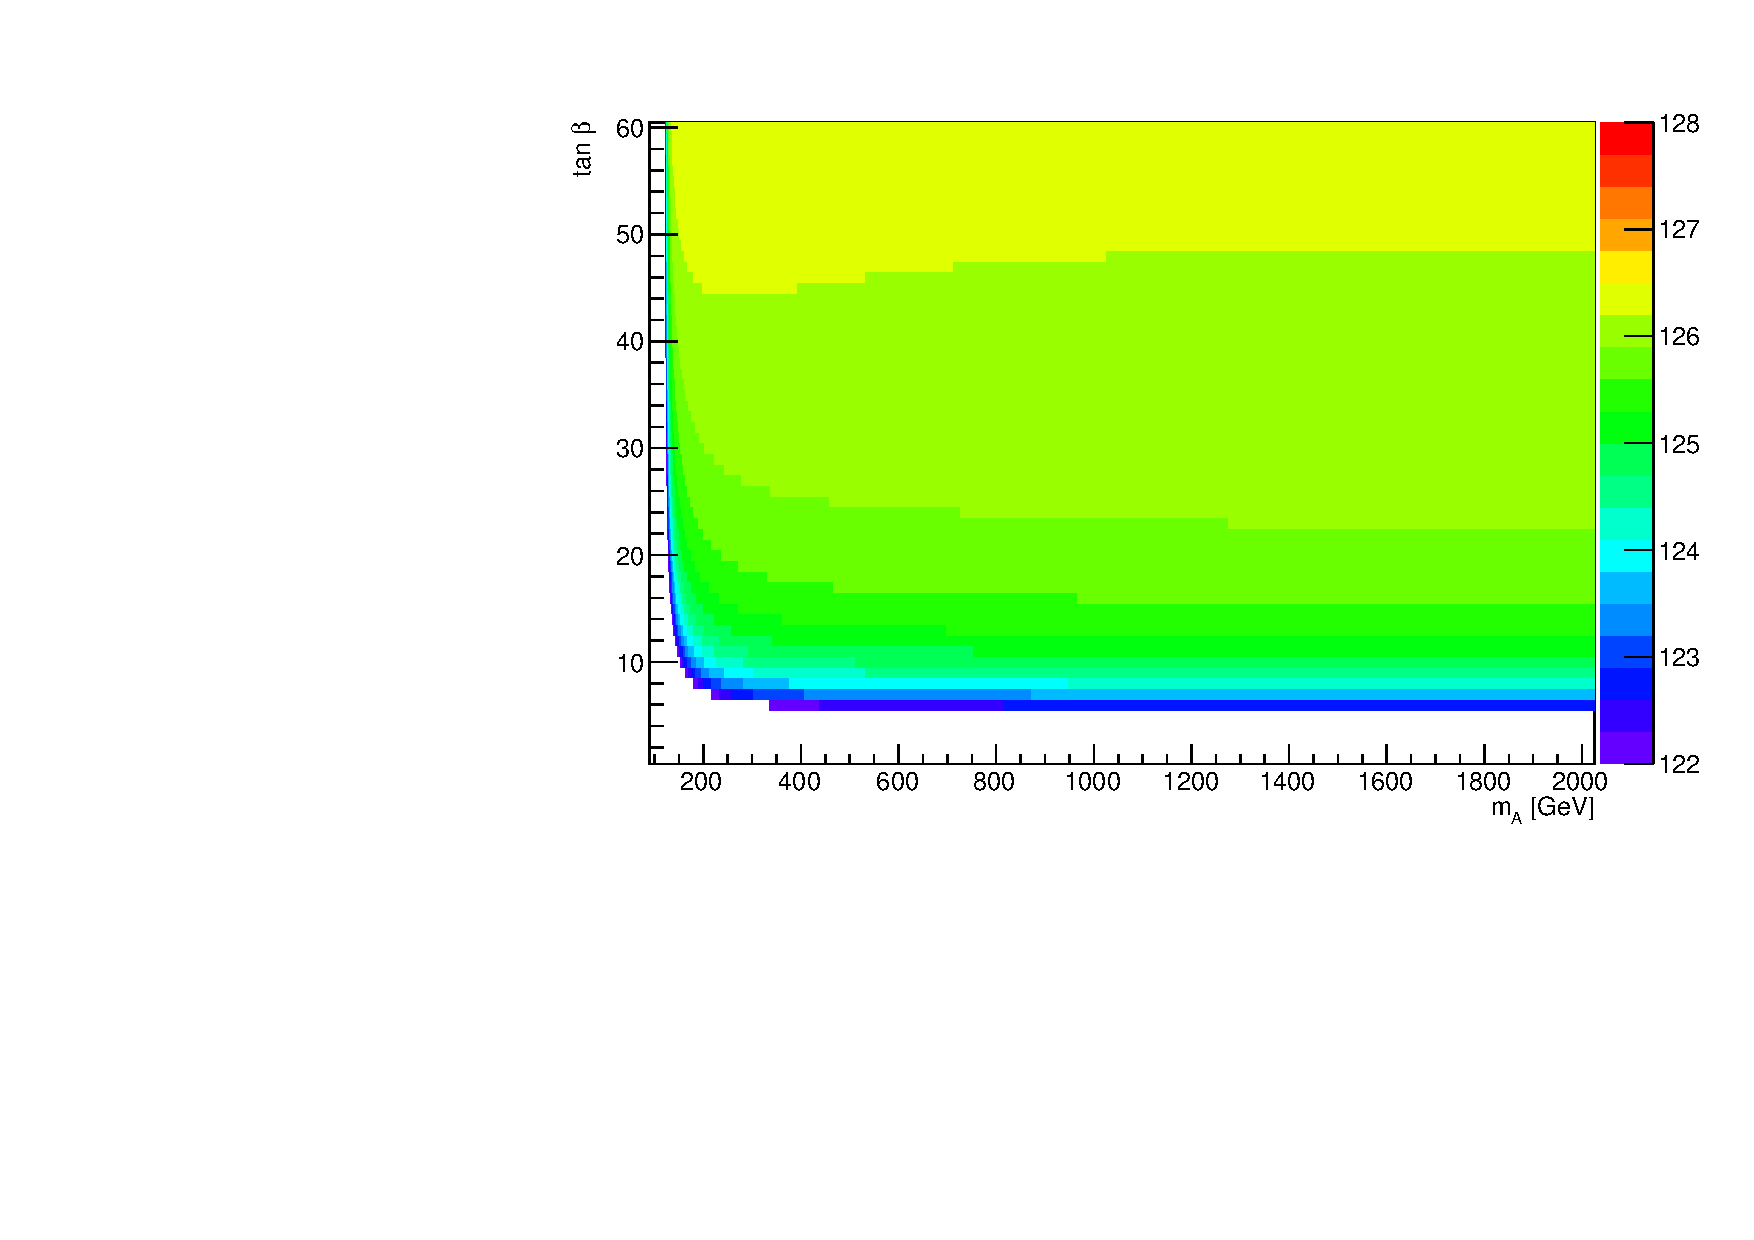
\includegraphics[width=0.5\textwidth]{./Theory/Figures/mh_mhmodp.pdf}
\end{center}
\caption{The mass of the light Higgs boson, \mh, as a function 
of \mA~and \tanb~in the $m_{h}^{\text{mod+}}$ scenario. The white areas
indicate masses lower than 122 GeV. The figure shows that
the mass of the light Higgs boson is compatible with 125 GeV over a large
part of the \mA-\tanb~plane.}
\label{fig:mhmodp_mh}
\end{figure}

Figure \ref{fig:mhmodp_xs} shows the cross--sections of
gluon fusion production of the \PHiggs boson and (four--flavour scheme) b-associated
production of the \PHiggsps boson in the $m_h^{\text{mod+}}$ scenario. Gluon fusion 
production dominates at low \tanb, while b-associated production has a larger cross--section
at high \tanb.

\begin{figure}[h!]
\begin{center}
\subfloat[$\sigma(gg\rightarrow \PHiggs)$]{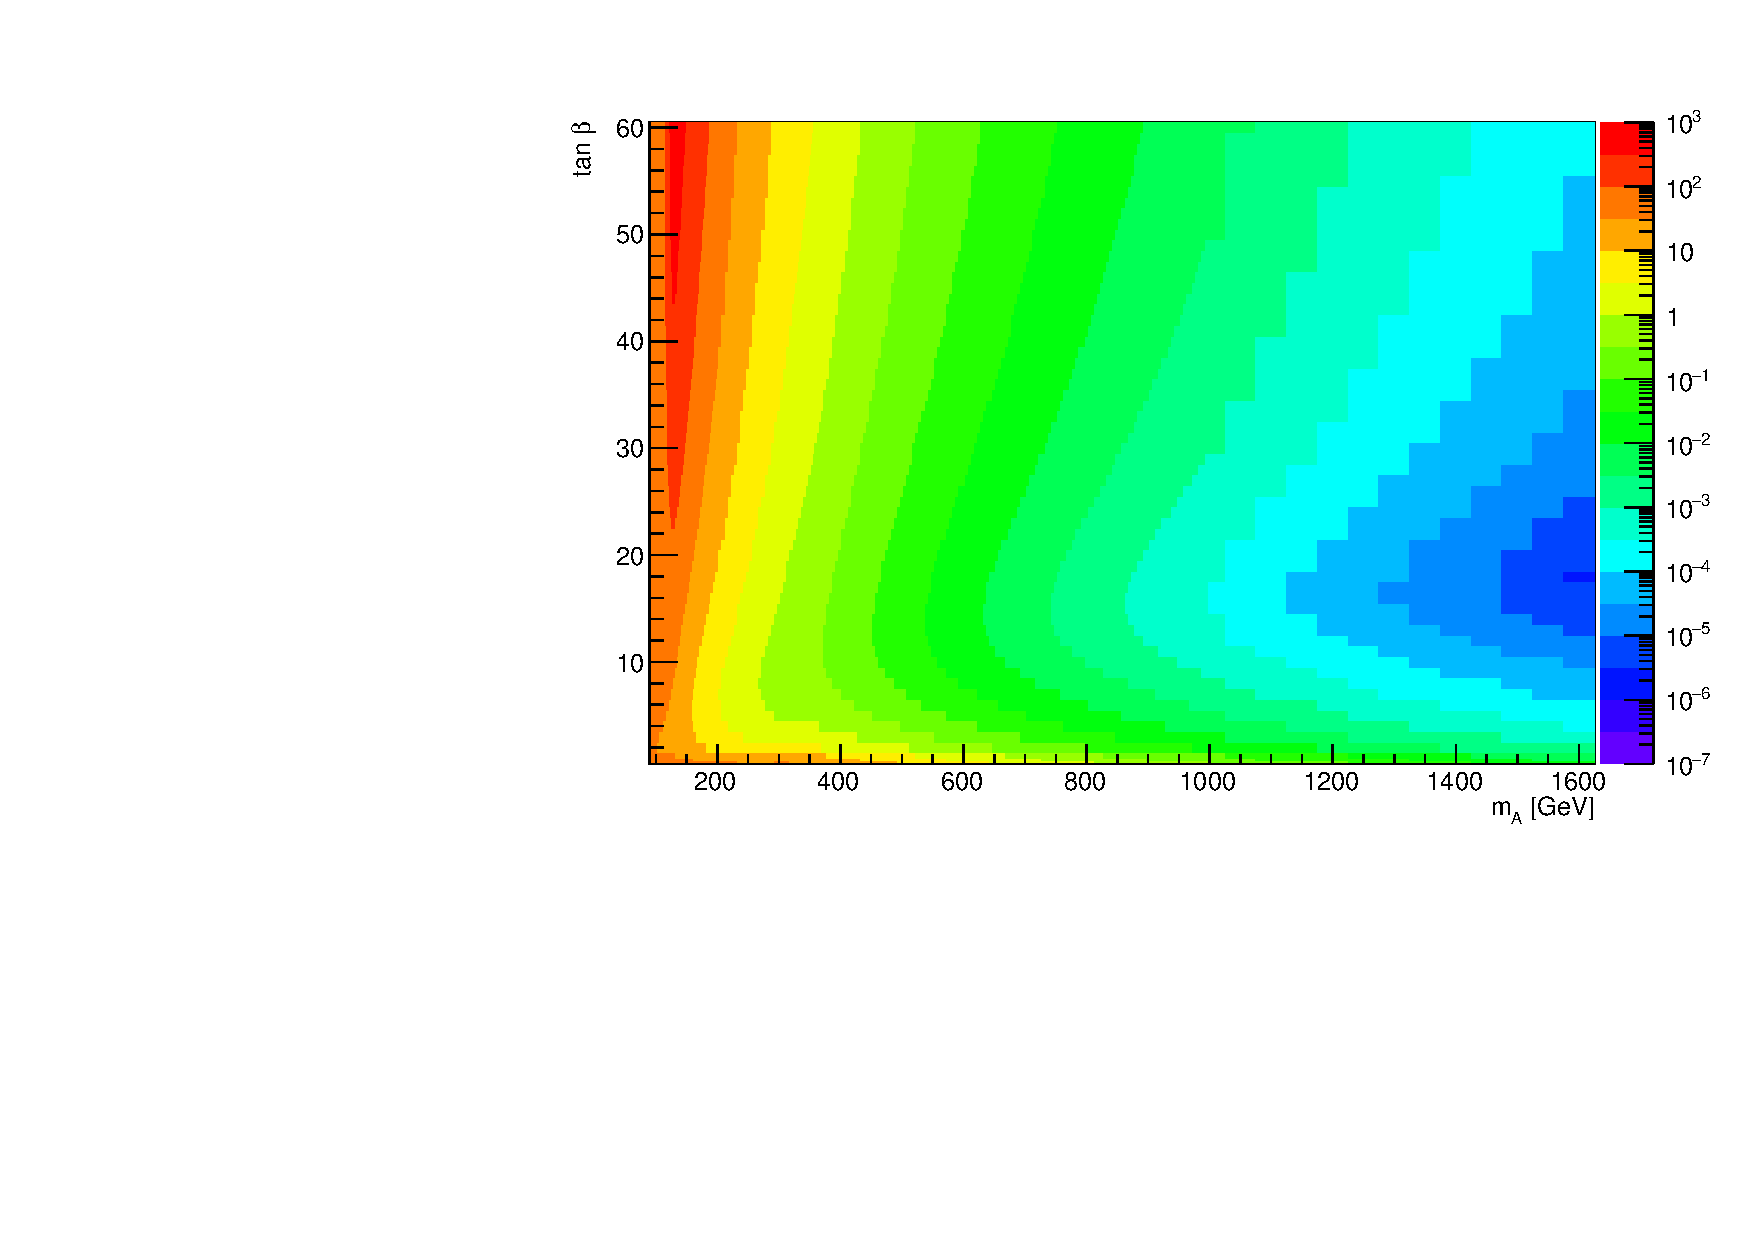
\includegraphics[width=0.5\textwidth]{./Theory/Figures/xs_ggH_mhmodp.pdf}}
\subfloat[$\sigma(gg\rightarrow bb\PHiggsps)$]{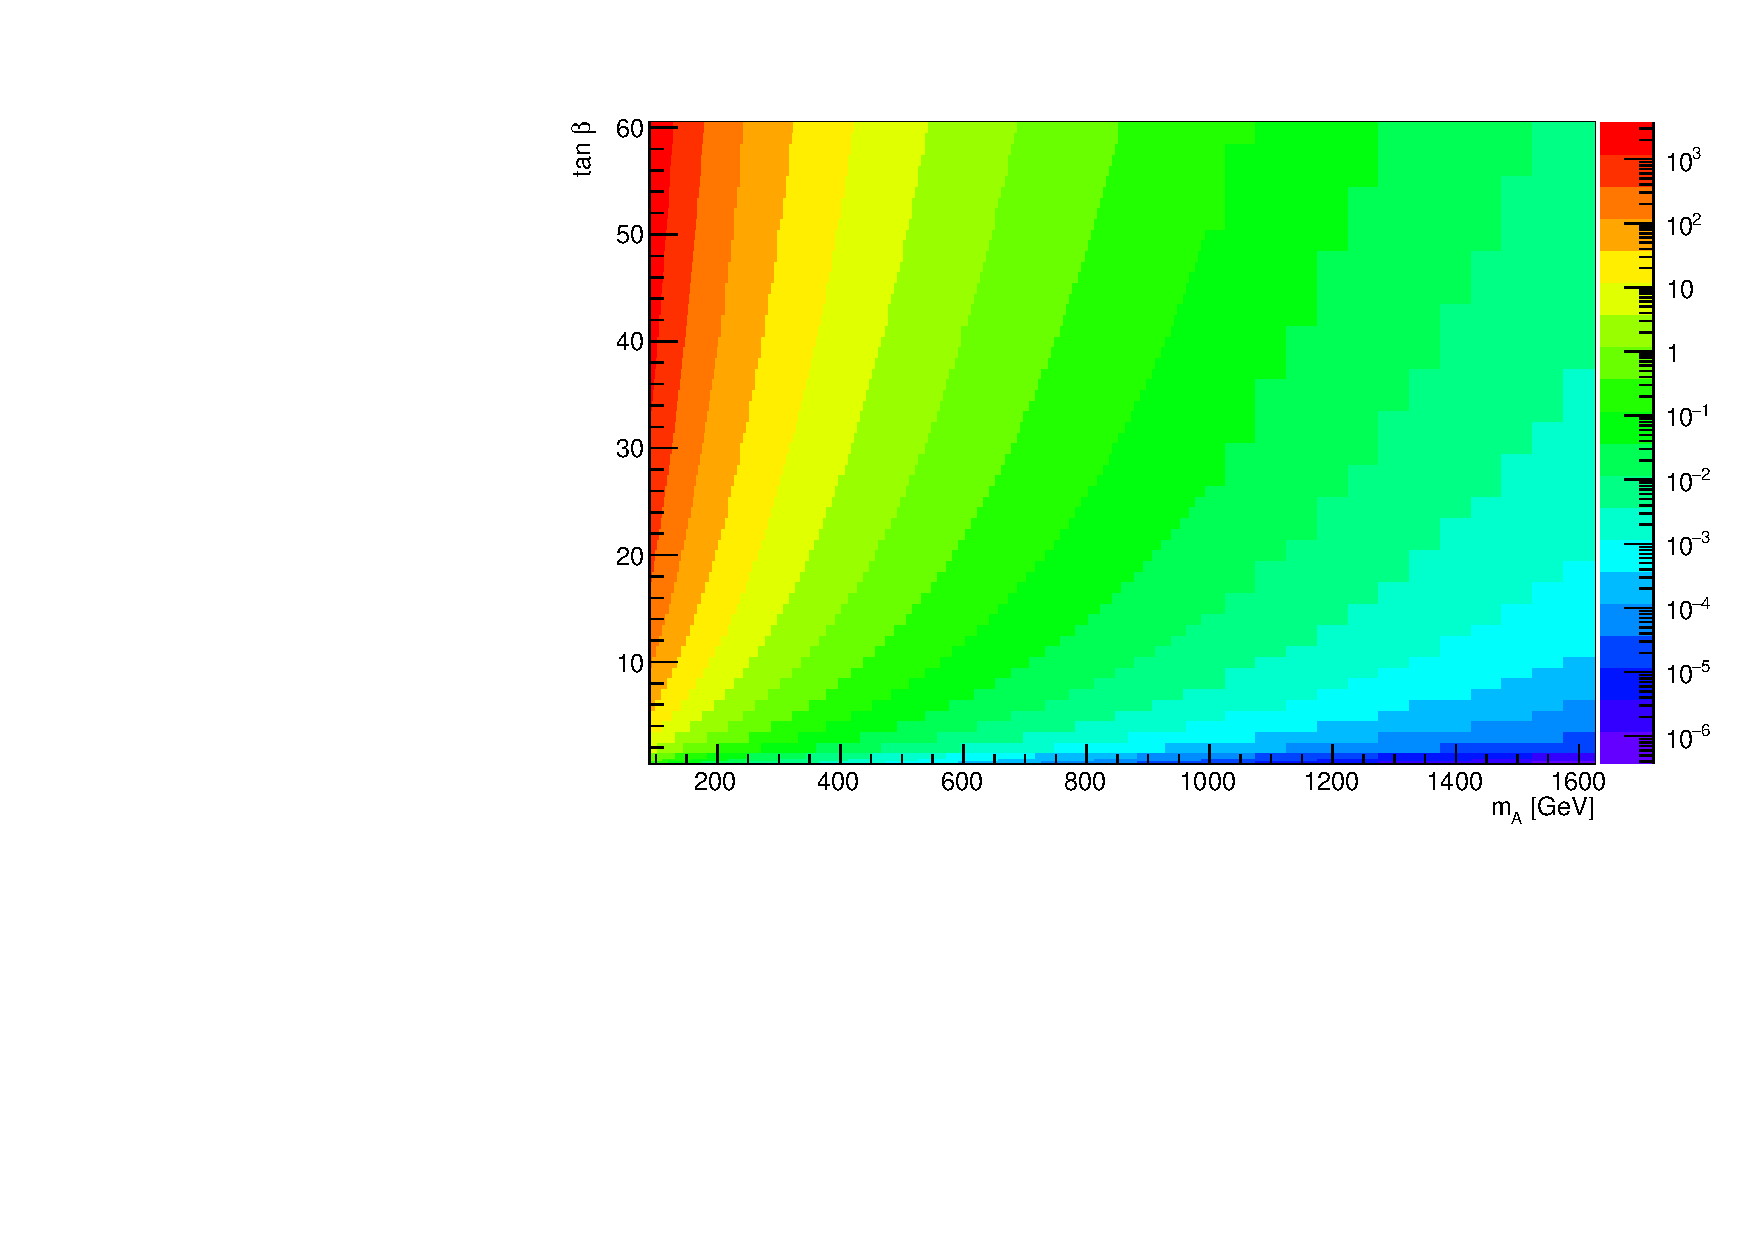
\includegraphics[width=0.5\textwidth]{./Theory/Figures/xs_bbA4FS_mhmodp.pdf}}
\end{center}
\caption{Production cross--section of (a) gluon fusion production of the \PHiggs boson and
(b) b--associated production (four--flavour scheme) of the \PHiggsps boson in the $m_{h}^{\text{mod+}}$ scenario. The gluon fusion production cross section is larger at low \tanb, while
the b-associated production cross-section is larger at high \tanb.}
\label{fig:mhmodp_xs}
\end{figure}

Figure \ref{fig:mhmodp_br} shows the branching ratio of the \PHiggs and \PHiggsps 
into $\tau\tau$. The branching ratios into $\tau\tau$ are enhanced, especially at
high \tanb, showing how this decay channel is useful for MSSM Higgs boson searches.

\begin{figure}[h!]
\begin{center}
\subfloat[BR($\PHiggs \rightarrow \tau\tau$)]{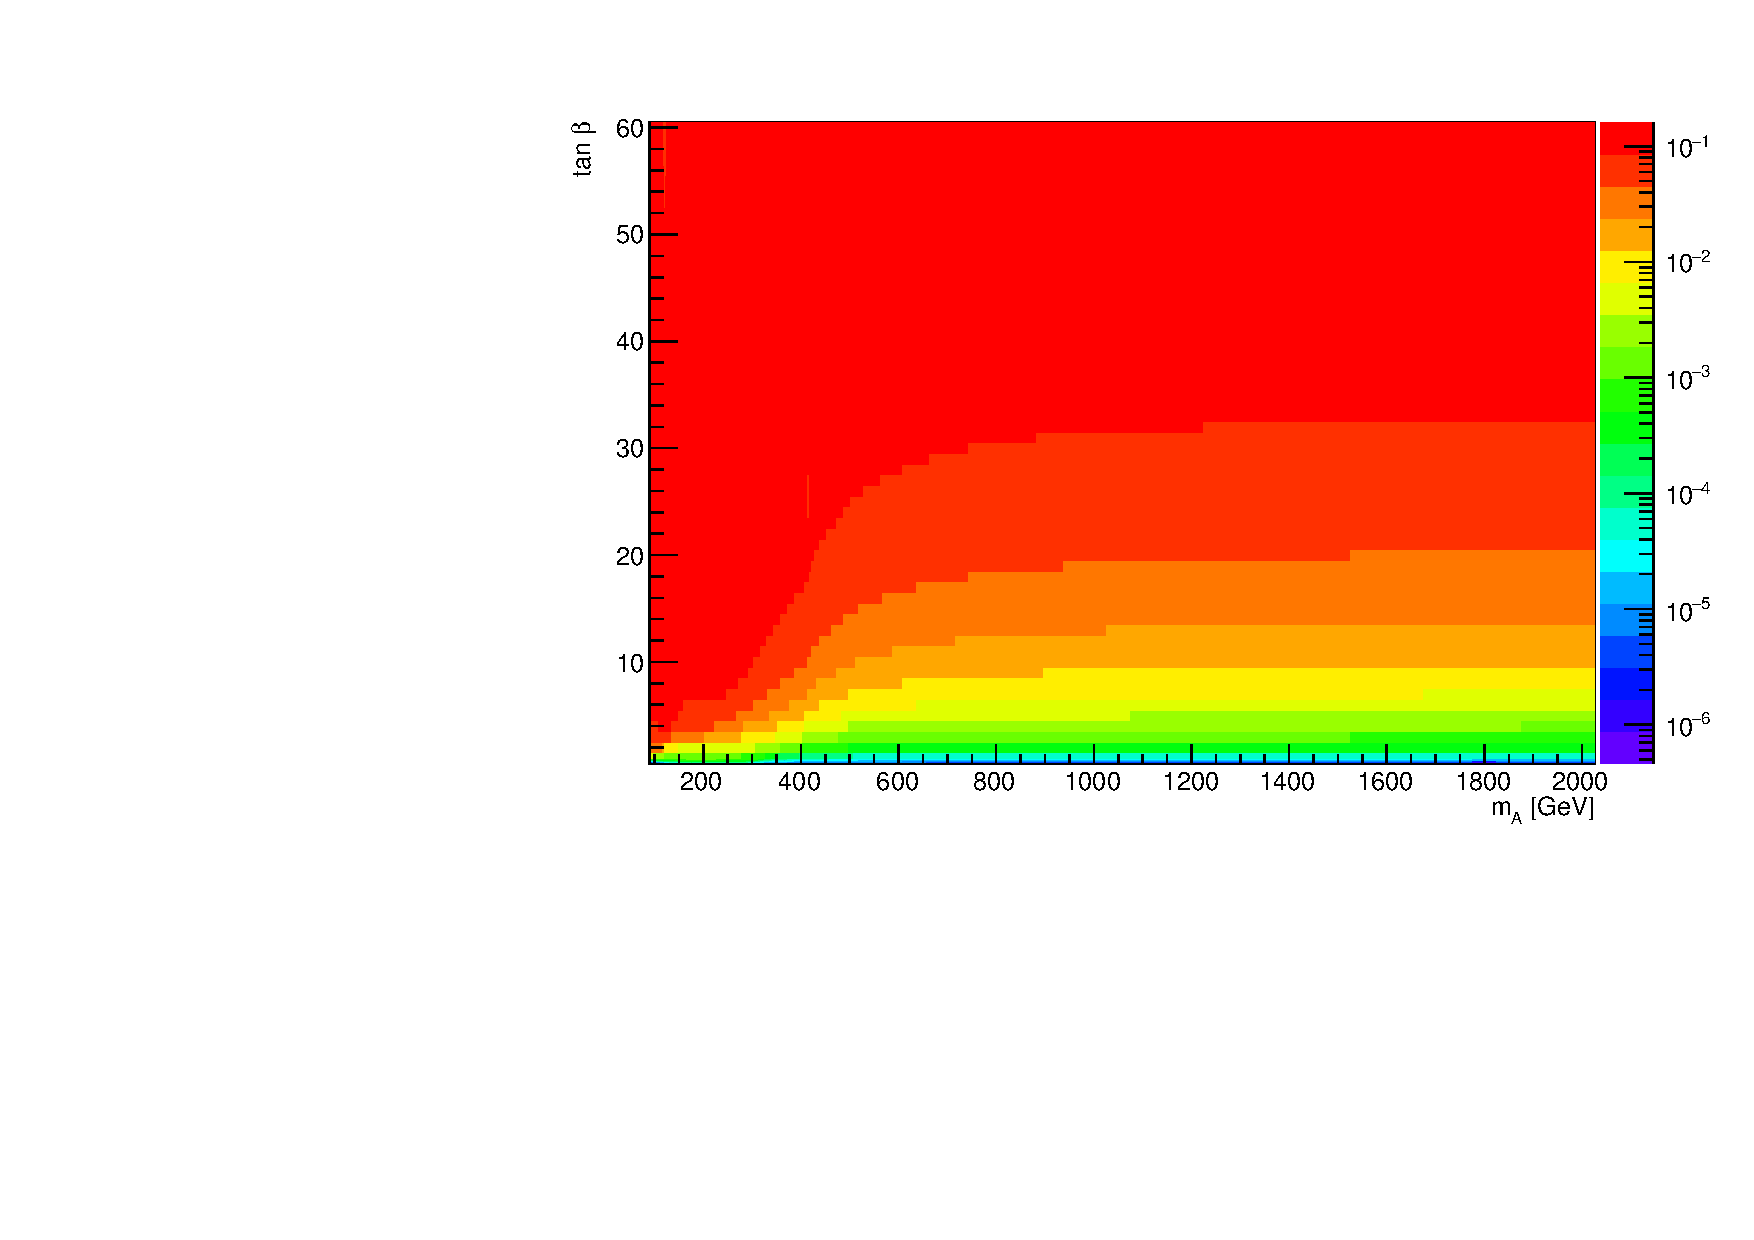
\includegraphics[width=0.5\textwidth]{./Theory/Figures/brHtautau_mhmodp.pdf}}
\subfloat[BR($\PHiggsps \rightarrow \tau\tau$)]{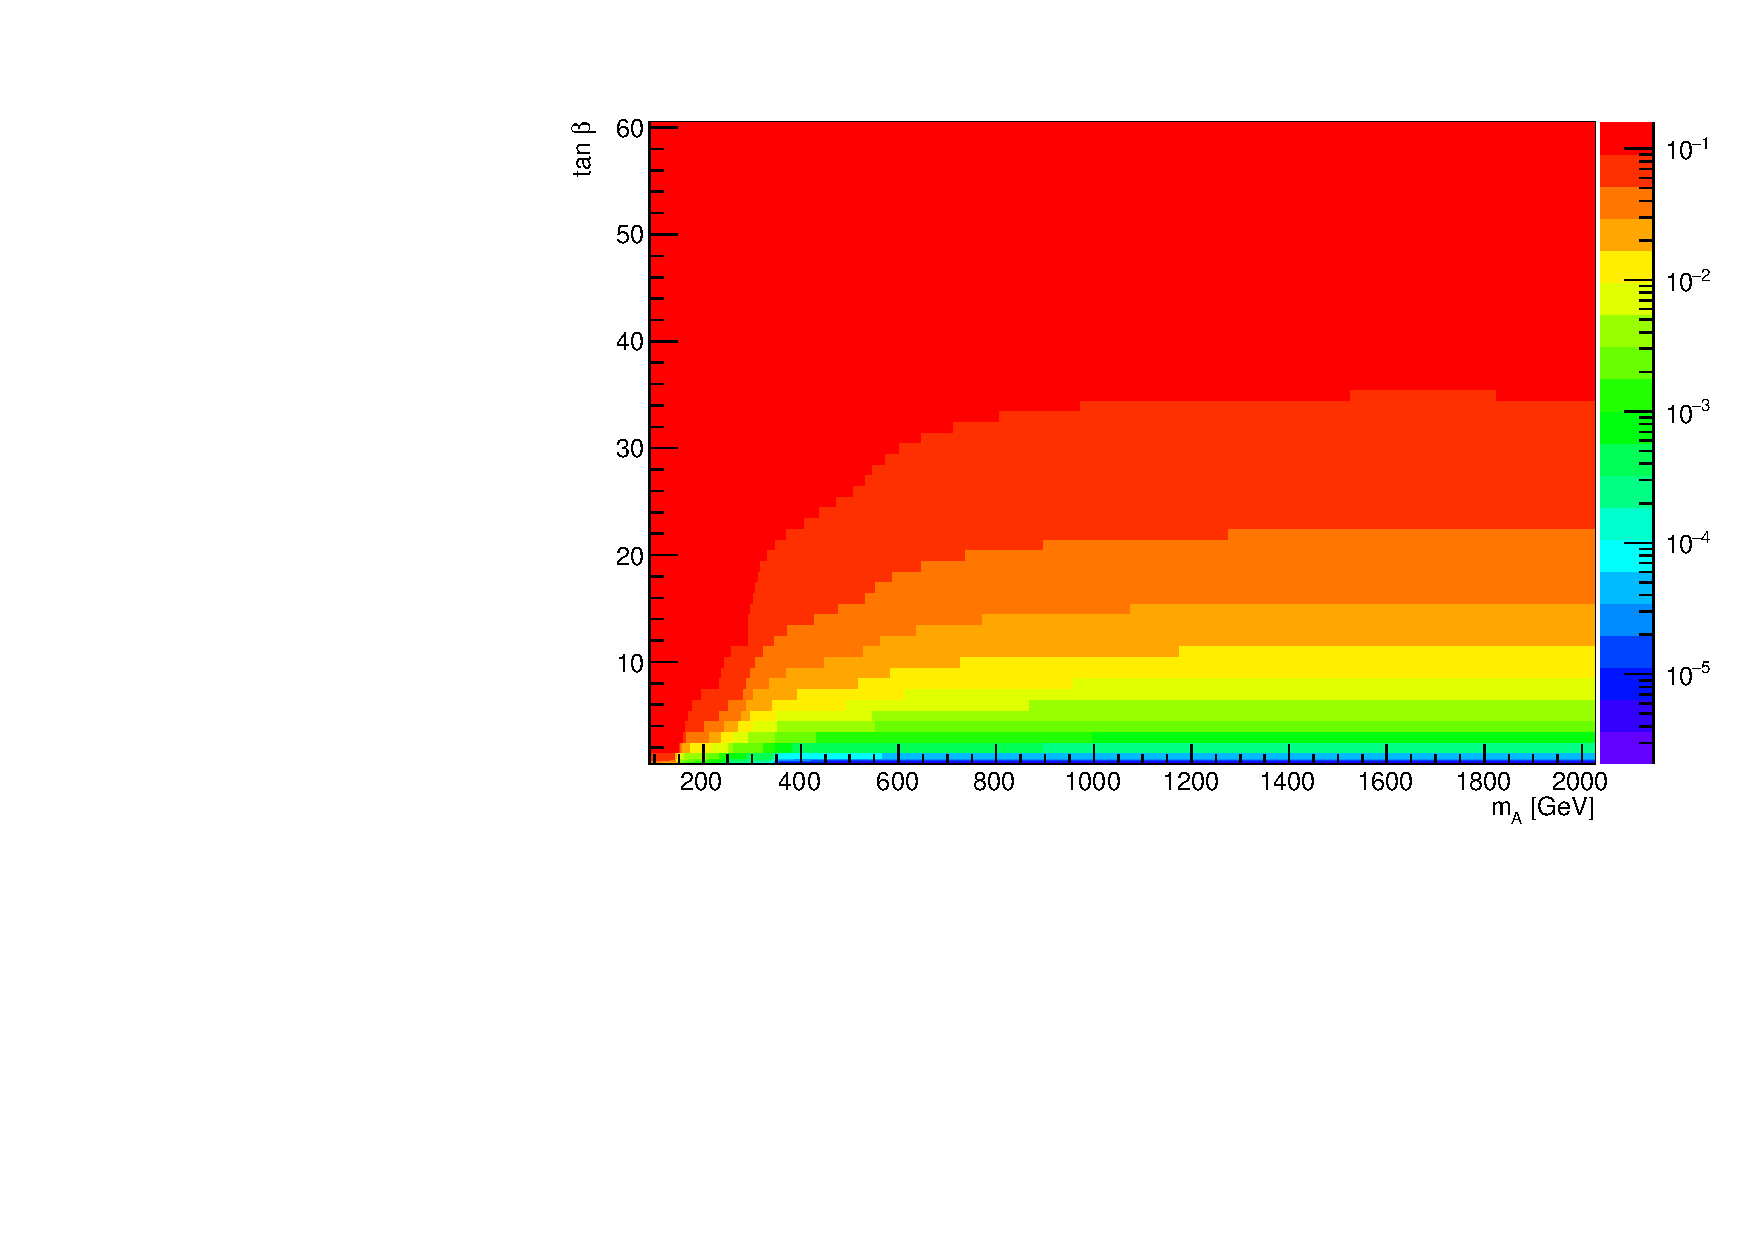
\includegraphics[width=0.5\textwidth]{./Theory/Figures/brAtautau_mhmodp.pdf}}
\end{center}
\caption{Branching ratio of (a) \PHiggs and (b) \PHiggsps into $\tau\tau$. The branching
ratios into $\tau\tau$ are enhanced at high \tanb.}
\label{fig:mhmodp_br}
\end{figure}


\subsection{MSSM scenarios at low \tanb}
\label{sec:mssm_theory_lowtb}
A large area of the \mA-\tanb~plane in the $m_{h}^{\text{mod+}}$ 
scenario contains a light Higgs boson with a mass compatible with
125 GeV. However, at low values of \tanb this is not the case, with
values of \mh~dropping below 122 GeV. The low \tanb~regime can be re-opened
if $M_{\text{SUSY}}$ is allowed to be greater than 3 TeV \cite{MSSM-reopen}. 
MORE ABOUT FINE-TUNING
%But not too large, see ref above!
Figure \ref{fig:tanb_accessibility} shows contours of constant
light Higgs boson mass as a function of \tanb~and $M_{\text{SUSY}}$.
It indicates that values of \mh~can be compatible with 125$\pm$3 GeV
for \tanb~values down to 1 if $M_{\text{SUSY}}$ is around 100-1000 TeV. 
\tanb~values of 3-5 are even accessible for $M_{\text{SUSY}}$ of around 10 TeV.

\begin{figure}[h!]
\begin{center}
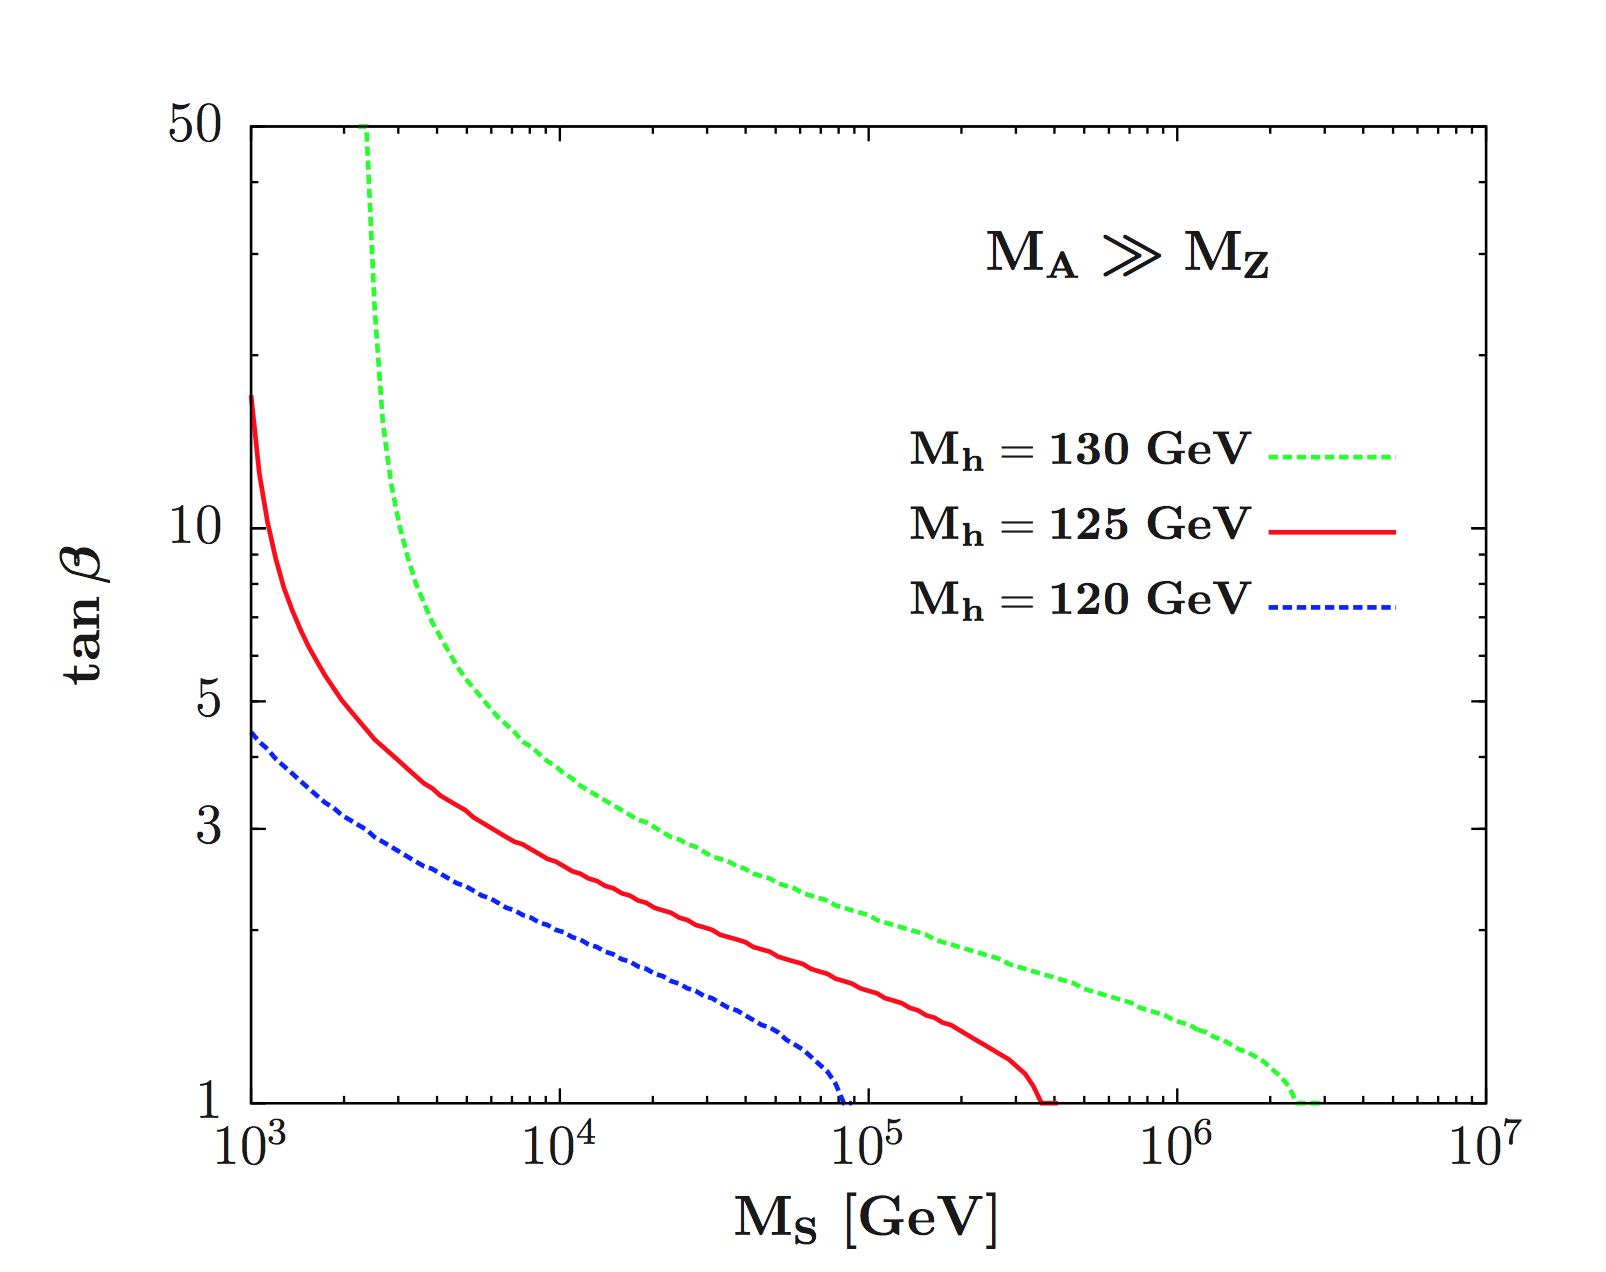
\includegraphics[width=0.5\textwidth]{./Theory/Figures/tanb_accessibility.png}
\end{center}
\caption{Contours of constant light Higgs boson mass as a function of \tanb~and $M_{\text{SUSY}}$.
High values of $M_{\text{SUSY}}$ allow for light Higgs boson masses compatible with
125 GeV down to low values of \tanb~\cite{hMSSM-2}.}
\label{fig:tanb_accessibility}
\end{figure}

%where the ±3 GeV variation corresponds to a rough estimate of the theoretical uncertainty of the MSSM prediction for mh, due to the unknown effect of higher-order correction

Two approches for the definition of an MSSM scenario that gives
access to the low-\tanb~region have been developed, they will be
discussed in the next sections.

\subsubsection{The low-\tanb-scenario}
\label{sec:theory_BSM_model_lowtb}
In the low-\tanb-scenario \cite{Hein-low-tb-high,MSSM-lowtanb}, the SUSY parameters entering
the radiative corrections are tuned to obtain light 
Higgs boson masses of around 125 GeV in most of the \mA-\tanb~plane considered.
Figure \ref{fig:lowtbhigh_mh} shows that, apart from in a corner of \tanb~1-4 and 
\mA~150-250 GeV, \mh~is compatible with 125 GeV.

\begin{figure}[h!]
\begin{center}
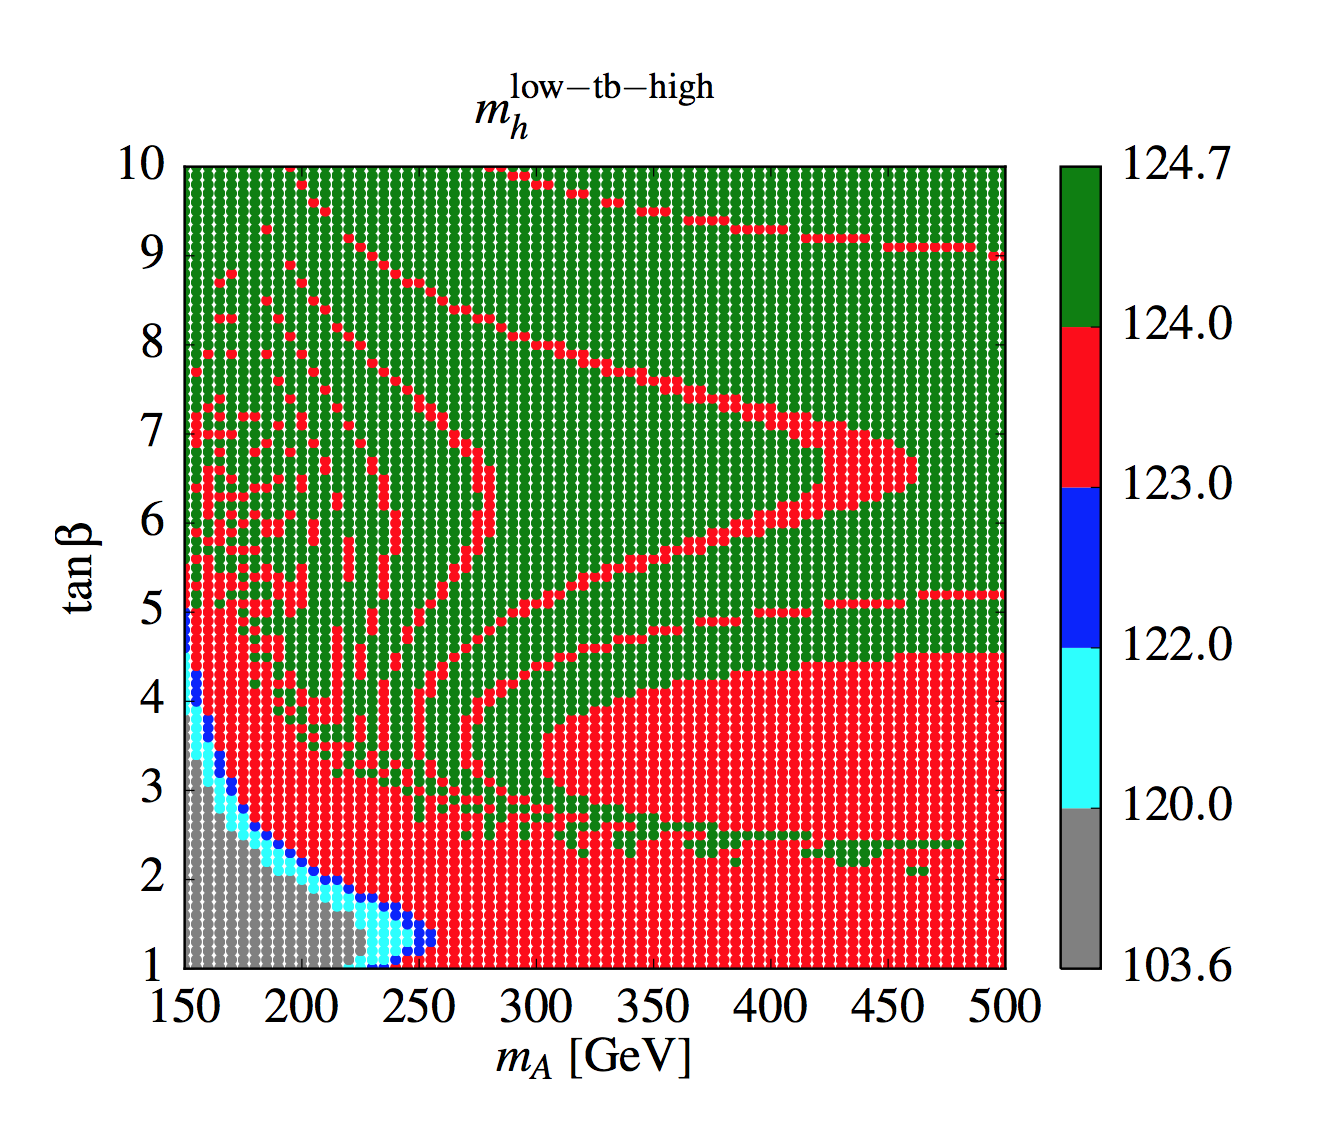
\includegraphics[width=0.5\textwidth]{./Theory/Figures/mh_lowtbhigh.png}
\end{center}
\caption{Mass of the light Higgs boson in the \mA-\tanb~plane of the low-\tanb~scenario.
The mass is compatible with 125 GeV nearly everywhere \cite{MSSM-lowtanb}.}
\label{fig:lowtbhigh_mh}
\end{figure}

To obtain \mh$\approx$125 GeV over a large part of the parameter
space, the SUSY parameters are chosen such that SUSY BREAKING MASSES ETC?
and $M_{\text{SUSY}}$ is not fixed but varies between a few TeV and 100 TeV, while
varying the parameter $X_t$ as:
\begin{equation}
\begin{split}
\tan{\beta} \leq 2 &: \frac{X_t}{M_{\text{SUSY}}} = 2\\
2 < \tan{\beta} \leq 8.6 &: \frac{X_t}{M_{\text{SUSY}}} = 0.0375\text{tan}^2\beta - 0.7\tan{\beta} + 3.25\\
8.6 < \tan{\beta} &: \frac{X_t}{M_{\text{SUSY}}} = 0.
\end{split}
\end{equation}
The other trilinear couplings are set to 2 TeV, with $\mu$ set to 1.5 TeV and $M_2$ to 2 TeV.

The branching fractions of \Htohh and \AtoZh in the low-\tanb~scenario are shown in
figure \ref{fig:lowtbhigh_br}. For both decay channels there are areas in the \mA-\tanb~plane
where the branching ratio is enhanced, indicating how analyses targeting such processes 
can be sensitive in this scenario. %REPHRASE
The analysis presented in chapter \ref{chap:hhh} is interpreted
in the low-\tanb~scenario.

\begin{figure}[h!]
\begin{center}
\subfloat[\Htohh]{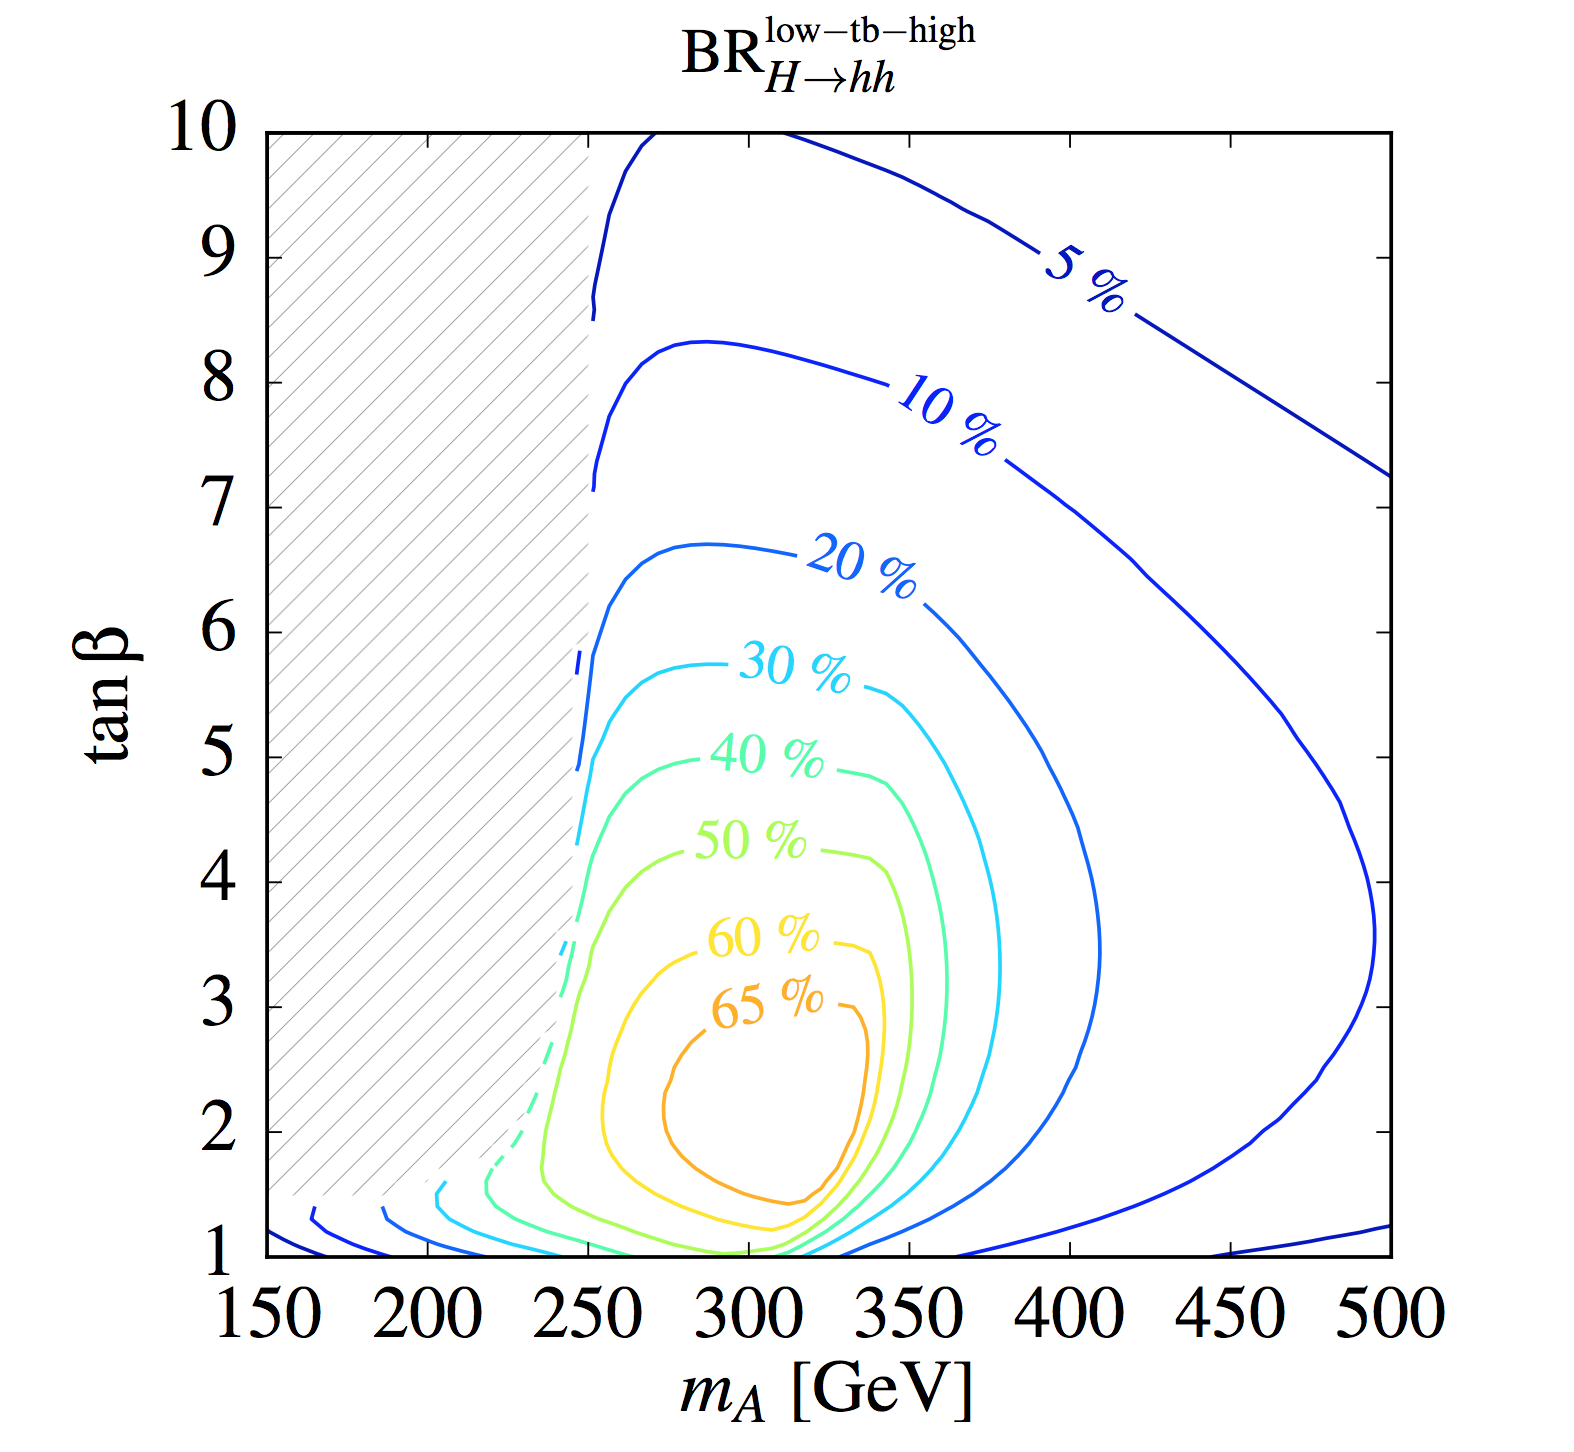
\includegraphics[width=0.5\textwidth]{./Theory/Figures/lowtbhigh_hhbr.png}}
\subfloat[\AtoZh]{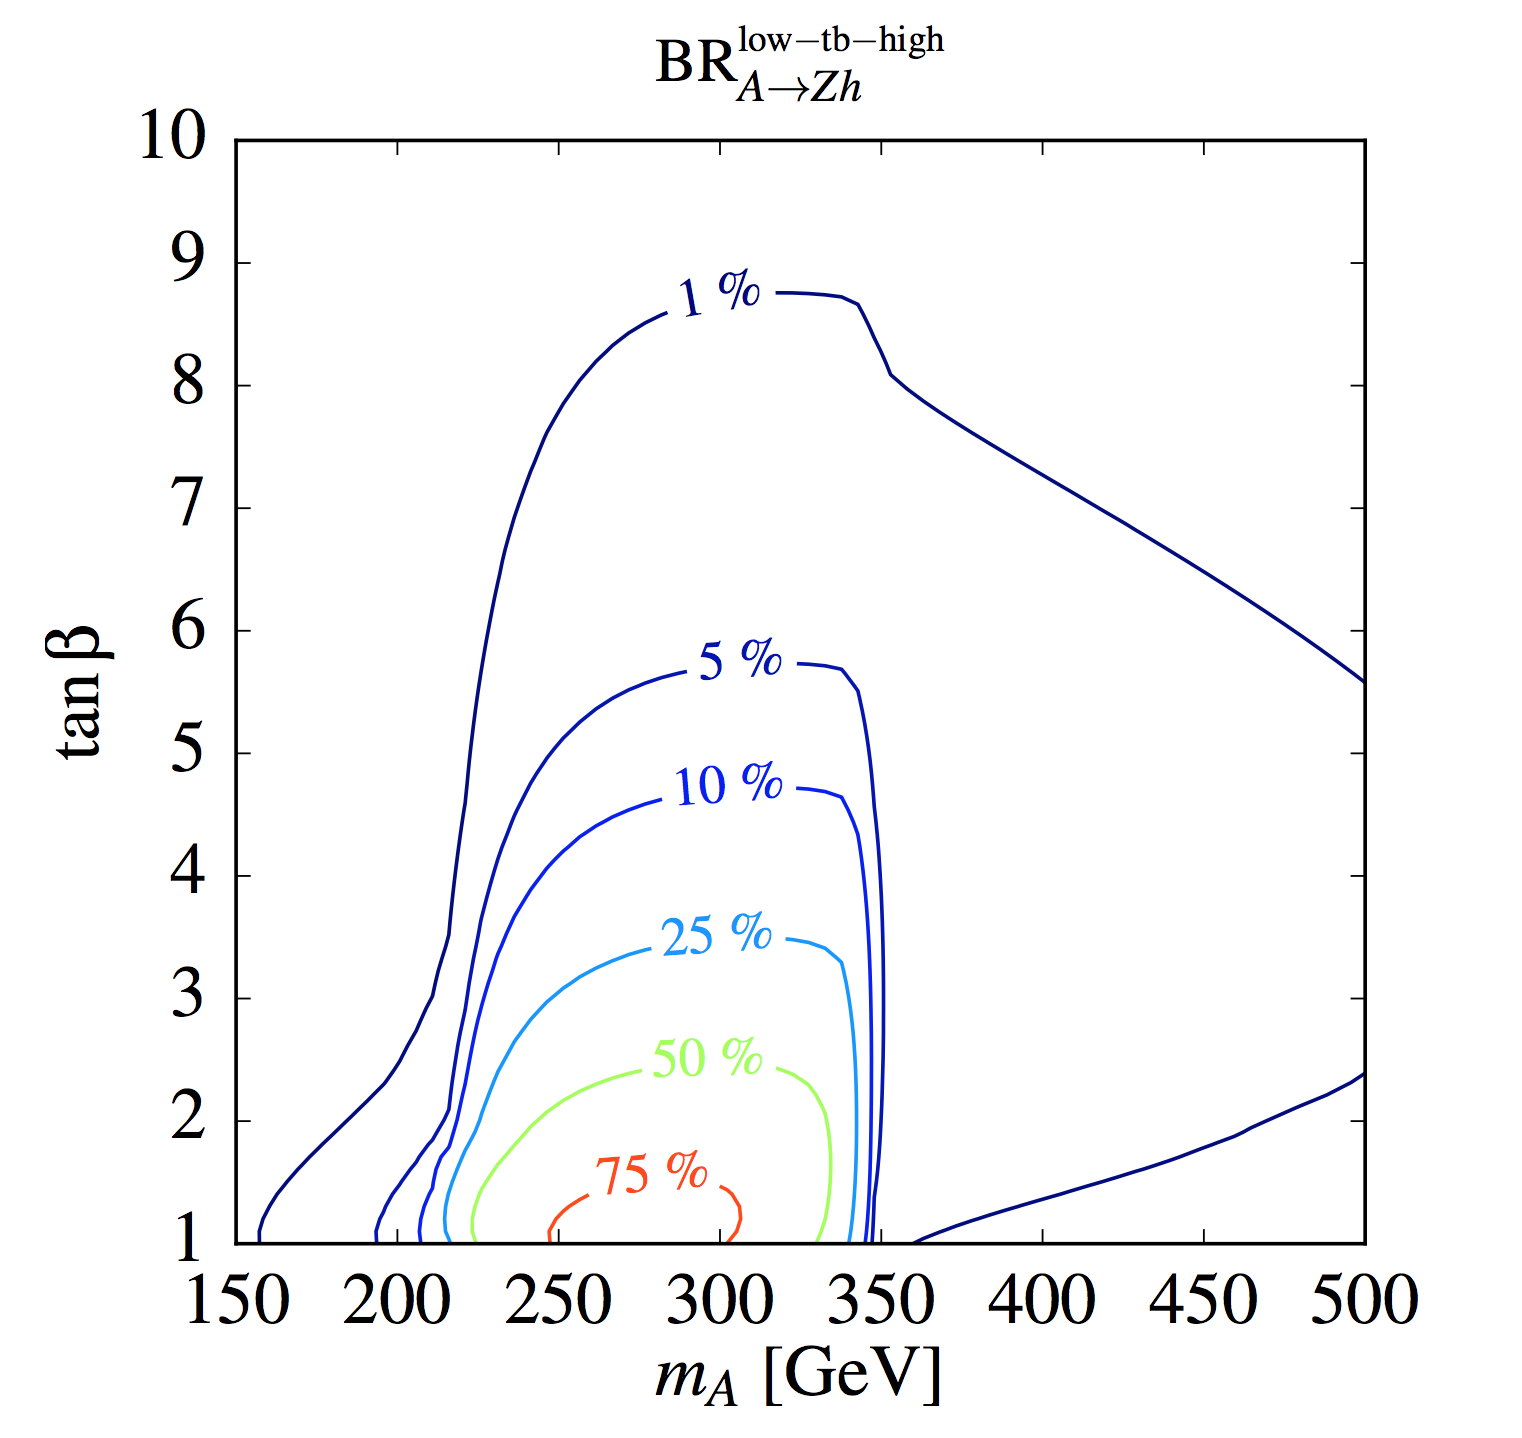
\includegraphics[width=0.5\textwidth]{./Theory/Figures/lowtbhigh_azhbr.png}}
\end{center}
\caption{Branching fractions of (a) \Htohh and (b) \AtoZh in the low-\tanb~scenario, indicating 
areas where both are significantly enhanced \cite{MSSM-lowtanb}.}
\label{fig:lowtbhigh_br}.
\end{figure}

\subsubsection{The hMSSM scenario}
\label{sec:theory_BSM_models_hMSSM}
The hMSSM scenario \cite{hMSSM-1,hMSSM-2} uses a different approach by starting from 
the REPHRASE tree-level expressions for masses and mixing and
the mass of the light Higgs boson \mh=125 GeV.

One of the assumptions of the hMSSM is that the
the mass matrix for the neutral CP-even states can
be decomposed as,
\begin{equation}
\label{eqn:hmssm_massmatrix}
\mathcal{M}^2_{\phi} = \mathcal{M}^2_{\text{tree}} + \begin{pmatrix}
\Delta\mathcal{M}^2_{11} & \Delta\mathcal{M}^2_{12} \\
\Delta\mathcal{M}^2_{12} & \Delta\mathcal{M}^2_{22} \end{pmatrix},
\end{equation}
where the $\Delta\mathcal{M}^2_{ij}$ are the radiative corrections.
The second assumption is that only $\Delta\mathcal{M}^2_{22}$ needs to be
taken into account, as this is the element that involves the stop-top correction
and so $\Delta\mathcal{M}^2_{22} >> \Delta\mathcal{M}^2_{12},\Delta\mathcal{M}^2_{11}$. 
Finally, all SUSY particles are assumed to be heavy enough not to be
detected at the \acs{LHC} and apart from effects on the mass matrix, 
the effects on the Higgs sector can be neglected.
%all SUSY particles are heavy enough to escape detection at the LHC, and their effects on the Higgs sector other than those on the mass matrix, e.g. via direct loop corrections to the Higgs-boson couplings or via modifications of the total decay widths, can be neglected.

Using these assumptions we can invert the lightest eigenvalue
of the mass matrix to get: 
\begin{equation}
\label{eqn:hmssm_deltam22}
\Delta\mathcal{M}^2_{22} = \frac{m_h^2(m_A^2+m_Z^2 - m_h^2) - m_A^2m_Z^2\text{cos}^22\beta}{m_Z^2\text{cos}^2\beta + m_A^2\text{sin}^2\beta - m_h^2},
\end{equation}

This means we can write,
\begin{equation}
\label{eqn:hmssm_mHalpha}
\begin{split}
&m^2_H = \frac{(m_A^2+m_Z^2-m_h^2)(m_z^2\cos{\beta}^2+m_A^2\sin{\beta}^2 - m_A^2m_Z^2\cos{2\beta}^2}{m_Z^2\cos{\beta}^2+m_A^2\sin{\beta}^2-m_h^2},\\
&\tan{\alpha} = -\frac{(m_Z^2+m_A^2)\cos{\beta}\sin{\beta}}{m_Z^2\cos{\beta}^2+m_A^2\sin{\beta}^2-m_h^2}.
\end{split}
\end{equation}
Combining this with the Hhh coupling,
\begin{equation}
\label{eqn:hmssm_Hhh}
\lambda_{Hhh} = \lambda_{Hhh,tree} + 3\frac{\Delta\mathcal{M}^2_{22}\sin{\alpha}}{m_Z^2\sin{\beta}}\cos{\alpha}^2,
\end{equation}
gives enough information to determine the cross sections and branching
ratios of all the five Higgs bosons as a function of \mA~and \tanb. The scenario
is only well defined in regions where the denominator in equations
\ref{eqn:hmssm_deltam22} and \ref{eqn:hmssm_mHalpha}, $m_Z^2\cos{\beta}^2+m_A^2\sin{\beta}^2 - m_h^2$, is nonzero. 
This leads to a minimum accesible \mA~value of \mh~at high \tanb, and
a minimum accessible \mA~of around 151 GeV for \tanb=1. In addition, the scenario
can be formulated, but is not strictly valid, for values of \tanb upwards of 10 \cite{CMS-PAS-HIG-16-007}.
The reason for this is that direct higher order SUSY corrections to down-type
fermion couplings and corrections due to SUSY particles in loops become relevant
above \tanb=10, but these are omitted in the hMSSM approach.

%to the couplings to the h, as expected from the SM, as will be further discussed in Section 3. This scenario is strictly valid for mA > 130 GeV and tanβ < 10. It can still be formulated for values up to tanβ < 60 though the omission of direct higher order SUSY corrections to down-type fermion couplings (also referred to as ∆β corrections) and corrections due to SUSY particles in loops, which be- come relevant for tan β > 10 question the consistency of the predictions with SUSY. A detailed

The production cross--sections at $\sqrt{s}=14$ TeV for gluon fusion production of the
H and A bosons, as well as for b-associated production, are shown in figure \ref{fig:hmssm_xs}.
As expected, gluon fusion production is dominant at low \tanb,with b-associated
production being more important at high \tanb. The cross sections increase for increasing \tanb,
apart from the gluon fusion cross section at low \tanb, where it decreases as \tanb~increases
due to a negative top-bottom intereference effect.

\begin{figure}[h!]
\begin{center}
\subfloat[$\sigma(gg\rightarrow\PHiggsps)$]{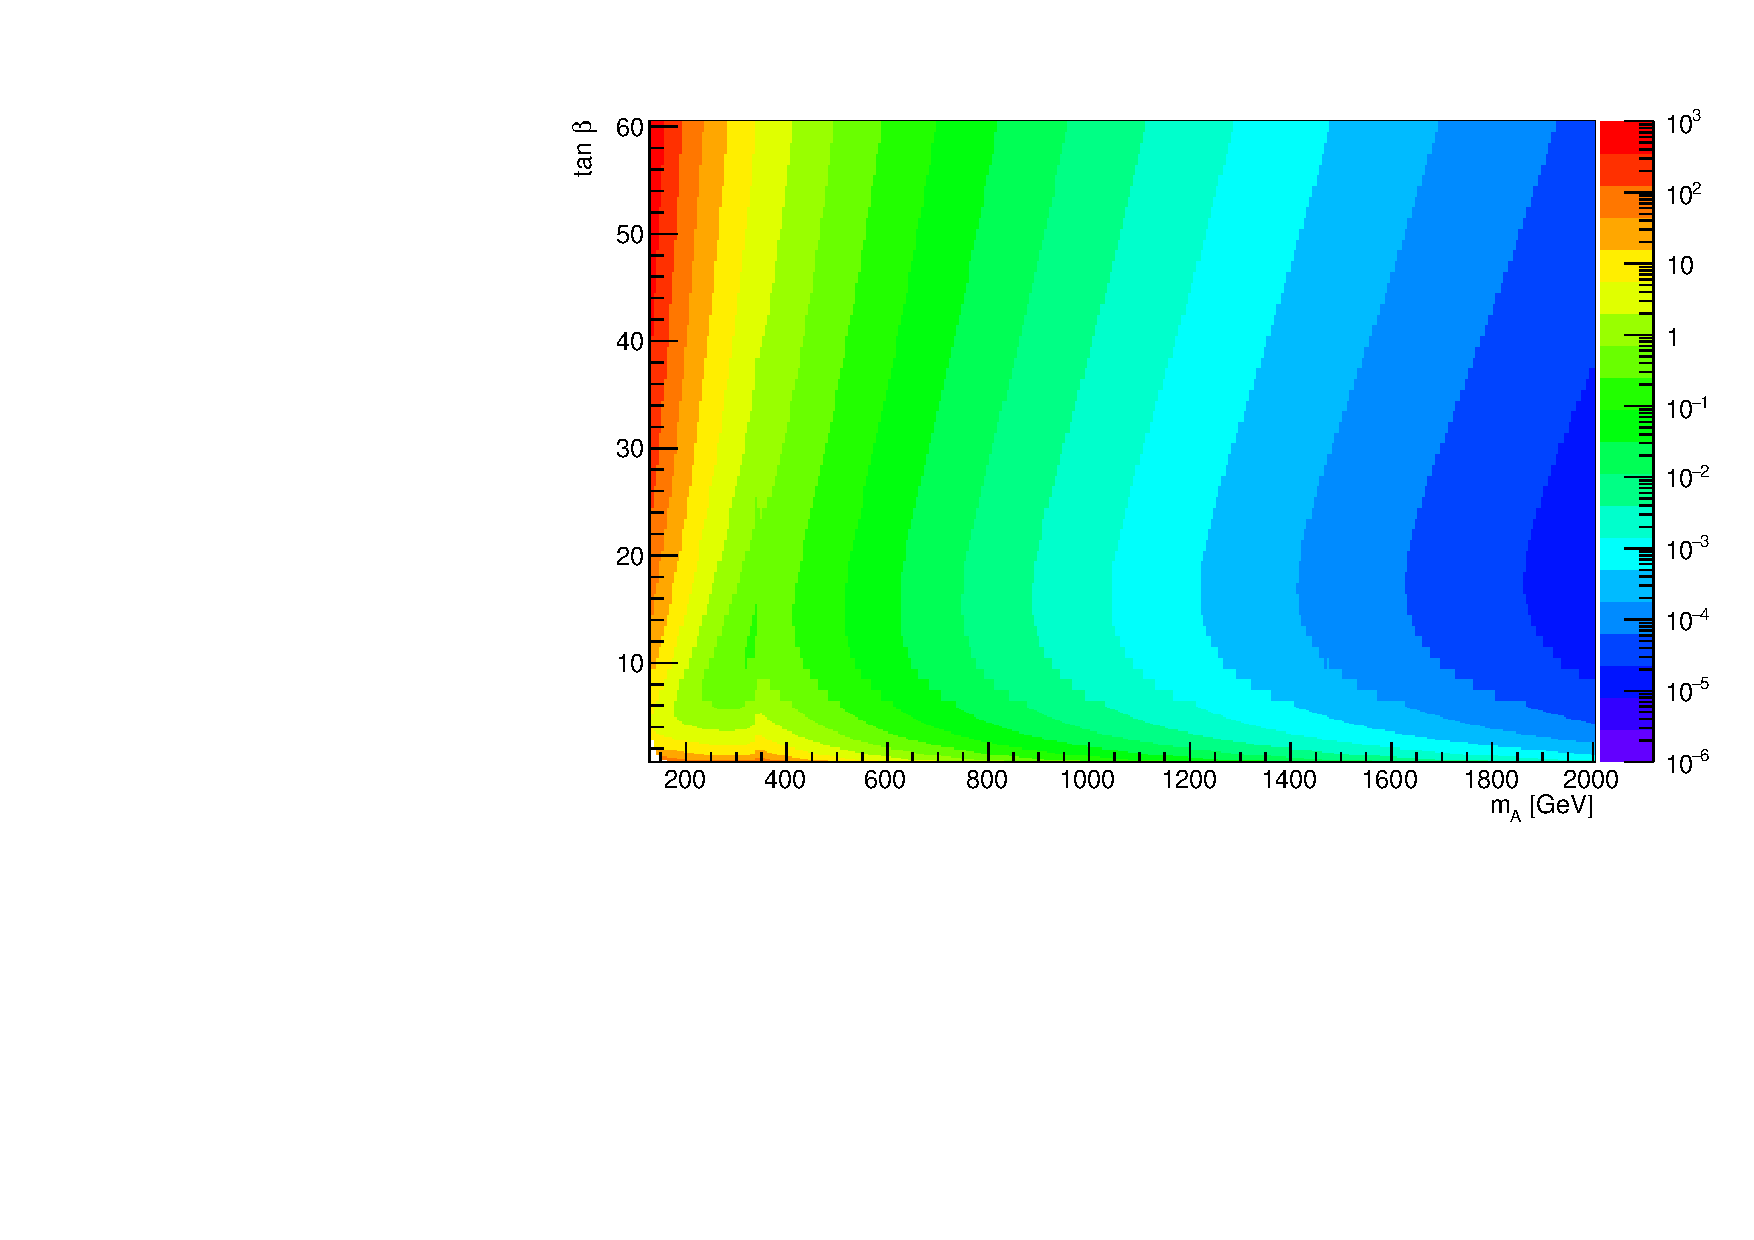
\includegraphics[width=0.5\textwidth]{./Theory/Figures/xsggA_hmssm.pdf}}
\subfloat[$\sigma(bb\rightarrow bb\PHiggs)$]{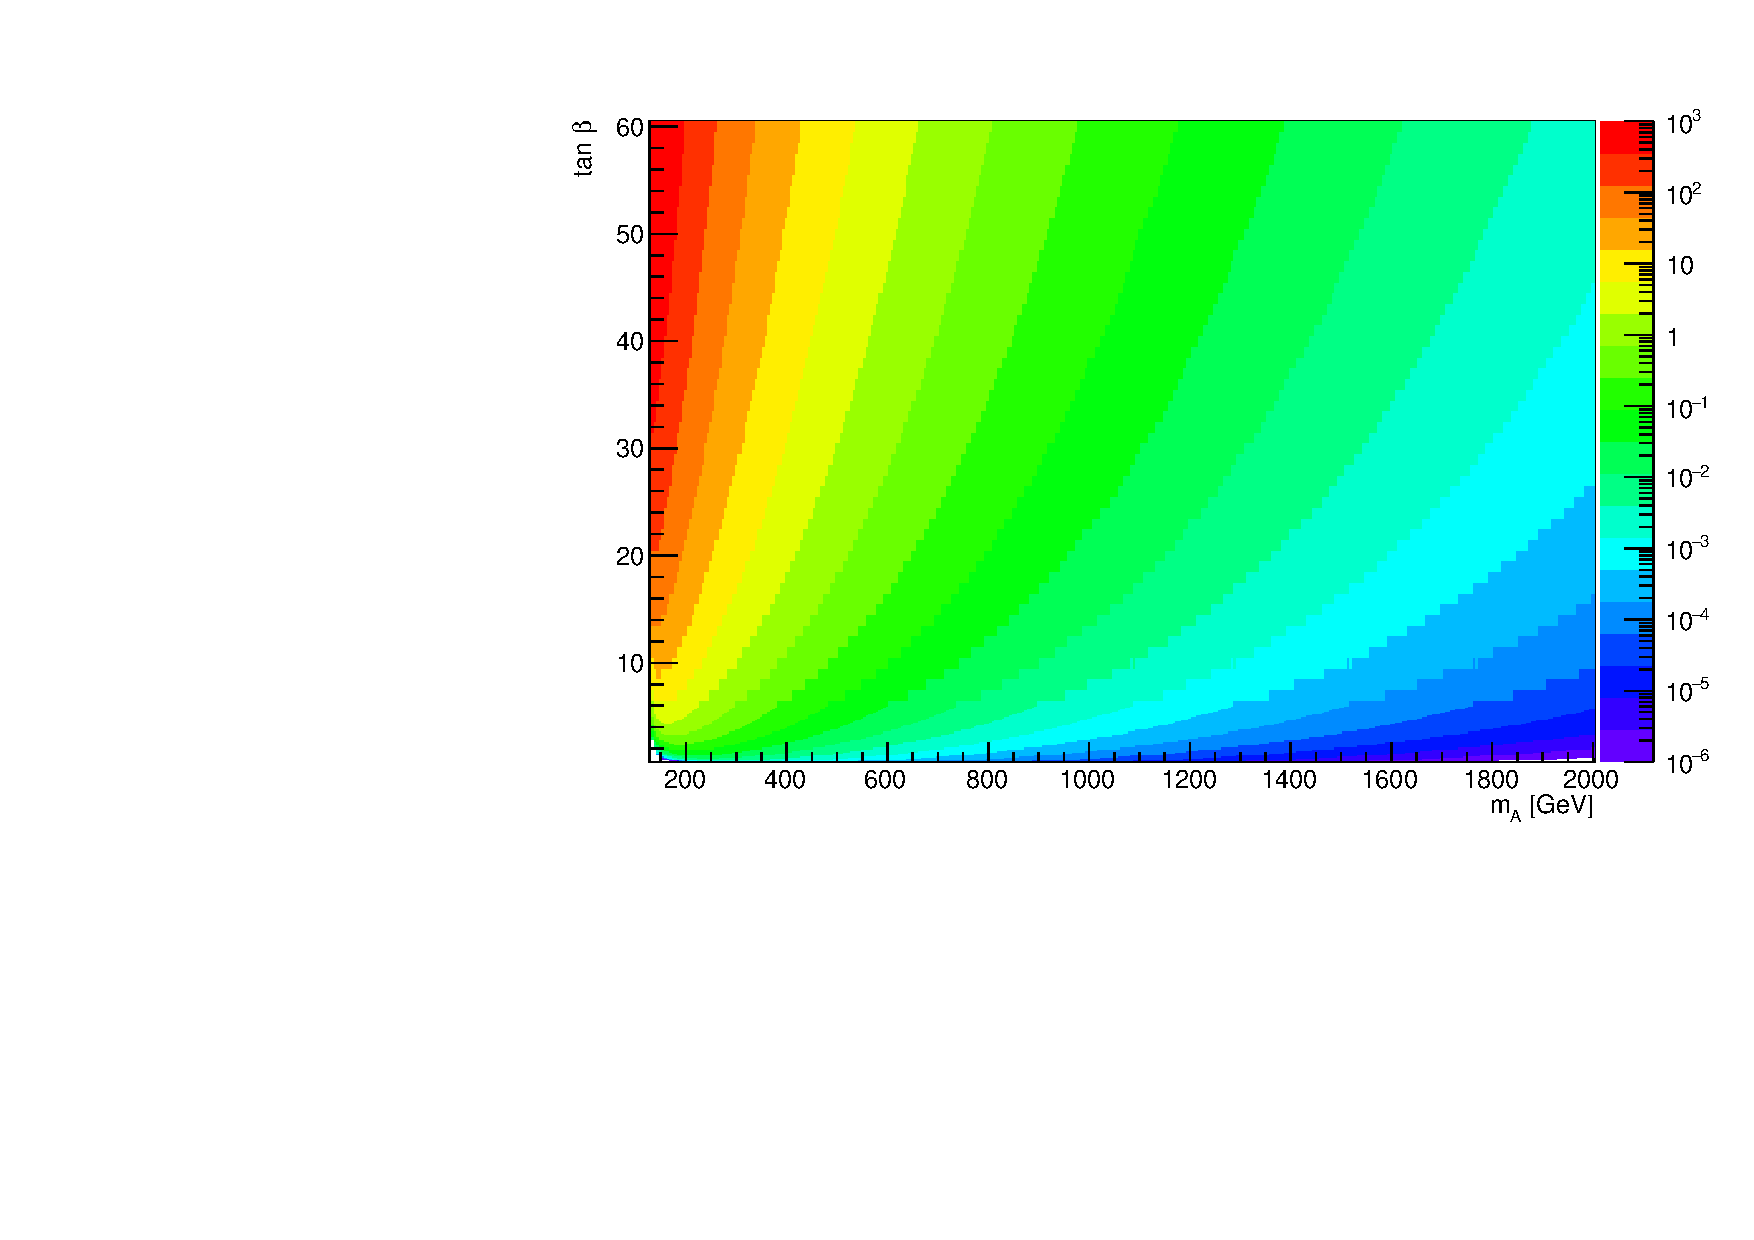
\includegraphics[width=0.5\textwidth]{./Theory/Figures/xsbbH4F_hmssm.pdf}}
\end{center}
\caption{Cross-sections at $\sqrt{s}=13$ TeV as a function of
\mA~and \tanb~ in 
the hMSSM scenario for (a) gluon fusion production of the \PHiggsps boson and (b)
b-associated production (four--flavour scheme) of the \PHiggs boson. We can generally see the cross-sections increase
with growing \tanb, apart from the gluon fusion cross section which decrease with increasing
\tanb~for low \tanb.}
\label{fig:hmssm_xs}
\end{figure}

Figure \ref{fig:hmssm_brtautau} shows the branching ratios of \PHiggsps and \PHiggs into \Pgt\Pgt.
The branching ratios are large over a large part of the mA-\tanb~plane, but mostly so
at high \tanb.

\begin{figure}[h!]
\begin{center}
\subfloat[BR$(\PHiggs\rightarrow\Pgt\Pgt)$]{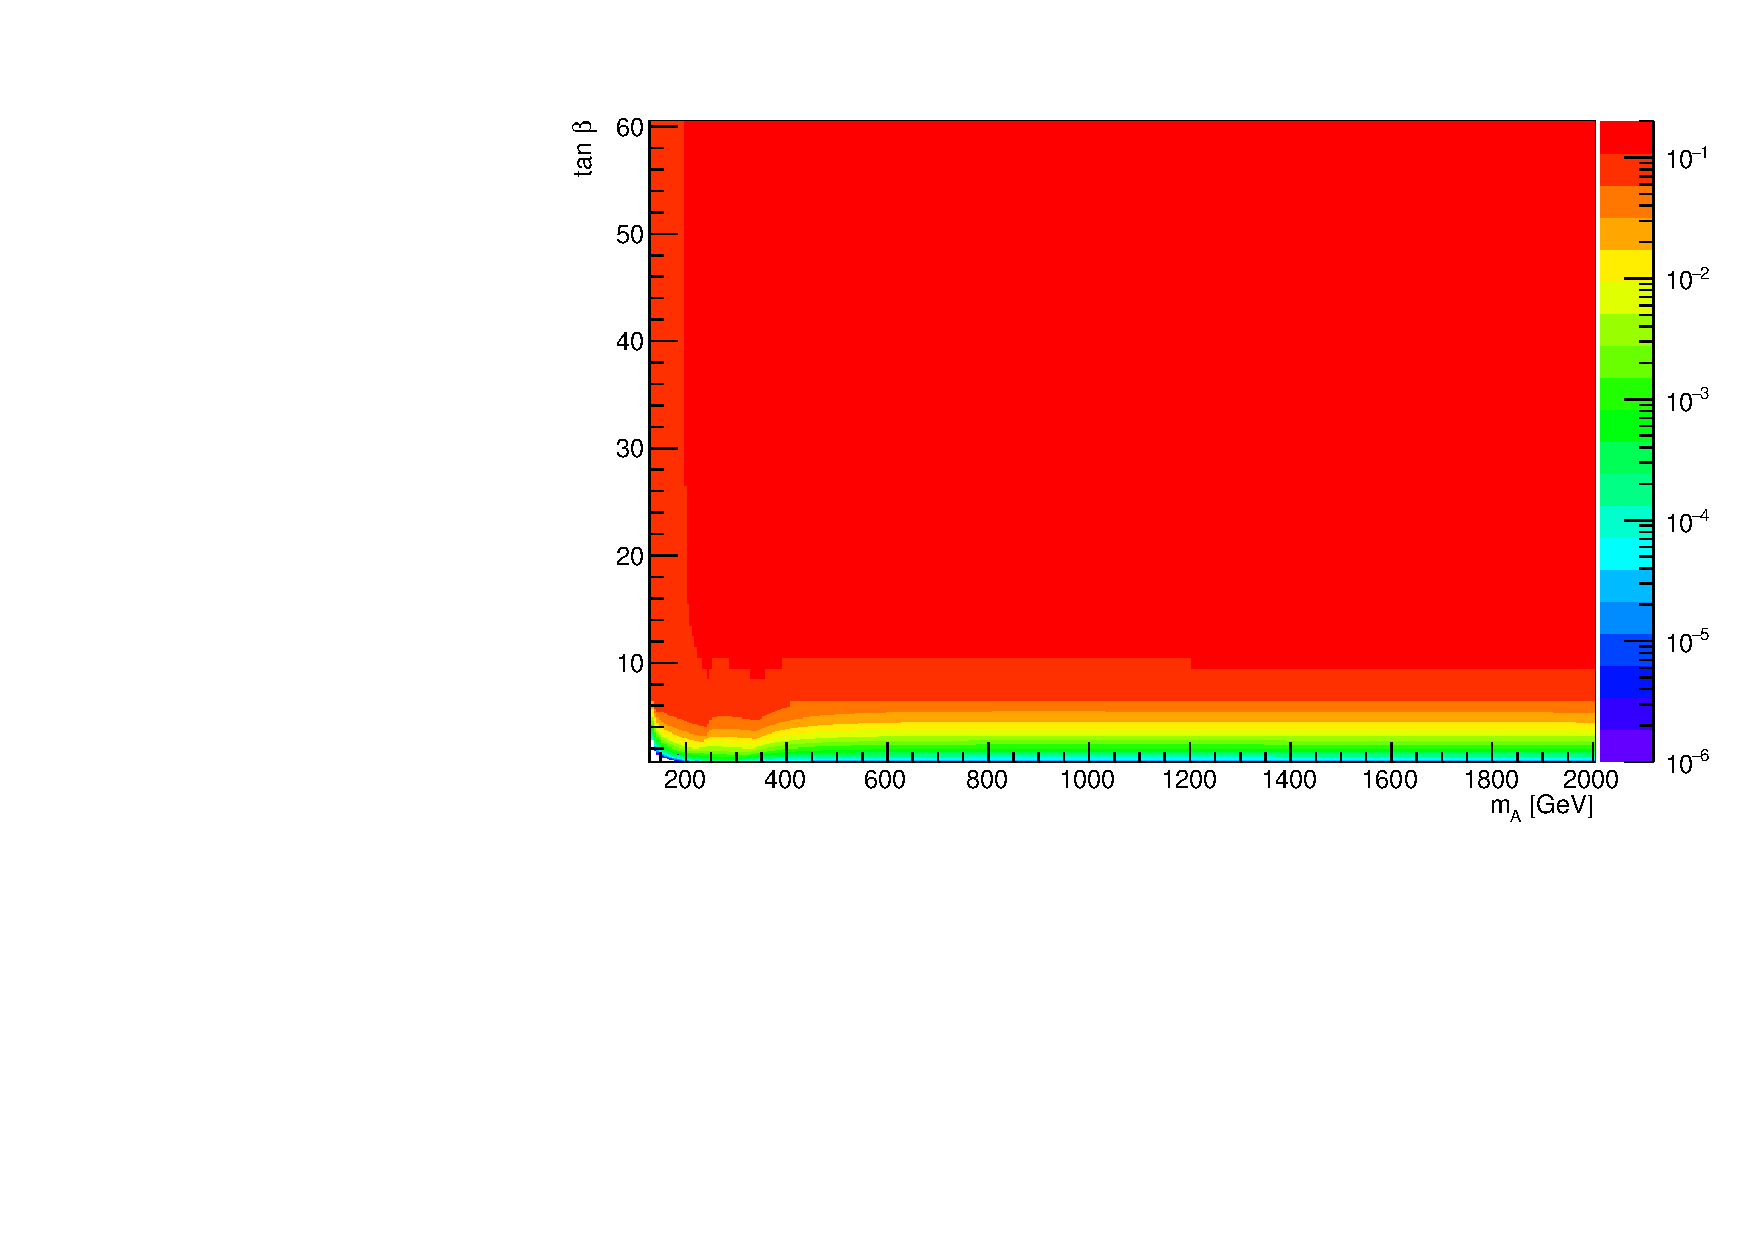
\includegraphics[width=0.5\textwidth]{./Theory/Figures/brHtautau_hmssm.pdf}}
\subfloat[BR$(\PHiggsps\rightarrow\Pgt\Pgt)$]{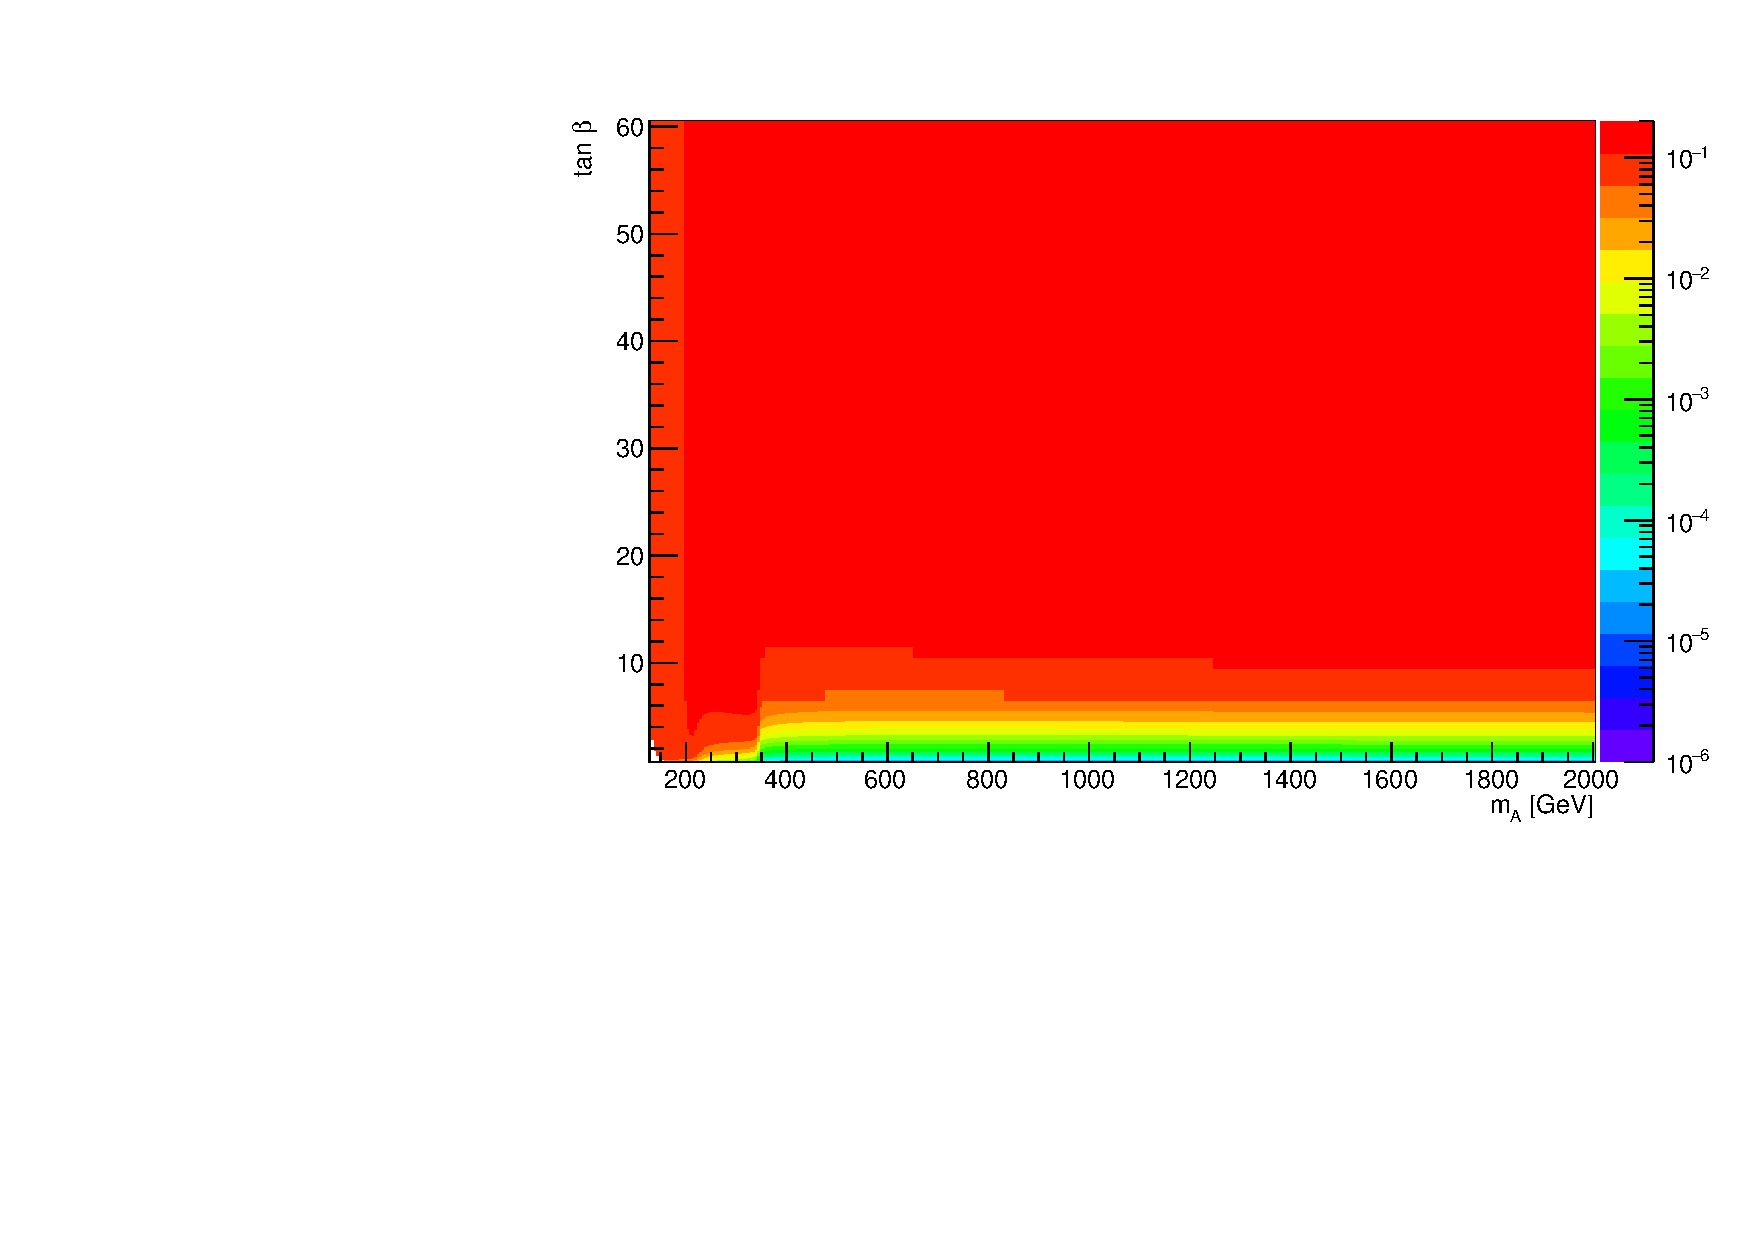
\includegraphics[width=0.5\textwidth]{./Theory/Figures/brAtautau_hmssm.pdf}}
\end{center}
\caption{Branching ratios of (a) the \PHiggs boson and (b) the \PHiggsps boson into \tautau. The
branching ratio is enhanced at high \tanb.} 
\label{fig:hmssm_brtautau}
\end{figure}


\section{Status of BSM Higgs boson searches}
\label{sec:theory_BSMH_status}
With the data collected during 
Run 1 of the \ac{LHC} many searches for BSM Higgs
bosons were already performed. The state of play with the full
Run-1 dataset collected by \ac{CMS} can be seen in figure \ref{fig:bsm_summary},
which shows the interpretations of different searches in the $m_{h}^{\text{mod+}}$ (figure \ref{fig:bsm_summary}a)
and hMSSM scenarios (figure \ref{fig:bsm_summary}b). The direct search for heavier Higgs bosons decaying into pairs
of tau leptons (shown in dark blue) sets the most stringent limits at high \tanb,with searches for 
heavy Higgs bosons decaying to $b\bar{b}$ and to $\mu\mu$ both excluding smaller parts of the high \tanb-region.
Searches for heavy Higgs bosons decaying to WW and ZZ are able to exclude part of the low-\tanb-region. In the 
hMSSM scenario searches for \Htohh and \AtoZh can exclude a small area at low \tanb~and between \mA=250-350 GeV.
The red exclusion contour in figure \ref{fig:bsm_summary}b is the re-interpretation of the analysis presented in
chapter \ref{chap:hhh}.

In Run-2 of the \ac{LHC} searches for \AHtotautau, setting more stringent limits than those shown in \ref{fig:bsm_summary},
have been performed in \ac{CMS}. The results of these searches will be presented in chapter \ref{chap:mssm}. 
Similar searches have been performed by \acs{ATLAS} \cite{ATLASMSSMtautau2016}. Neutral BSM Higgs bosons
are being searched for in other channels too, with some results for decays into \ttbar \cite{ATLASHttbar}, 
ZZ \cite{CMSHZZ2016,ATLASHZZ2016}, and WW \cite{ATLASHeavyHWW} already public.
In addition, searches for charged
Higgs bosons \cite{ATLASHplustaunu,ATLASHplustb,CMSHplustaunu} and
di-Higgs searches \cite{ATLASHbbgamgam,ATLASHgamgamWW,ATLASHhhbbbb,CMSbbgamgam,CMSHbbtautau,CMSHbbWW}, both in 
various final states, have been performed. The interest in these searches will remain, and so
as more data are collected during Run 2 more of such searches will be performed.

\begin{figure}[h!]
\begin{center}
\subfloat[$m_{h}^{\text{mod+}}$ scenario]{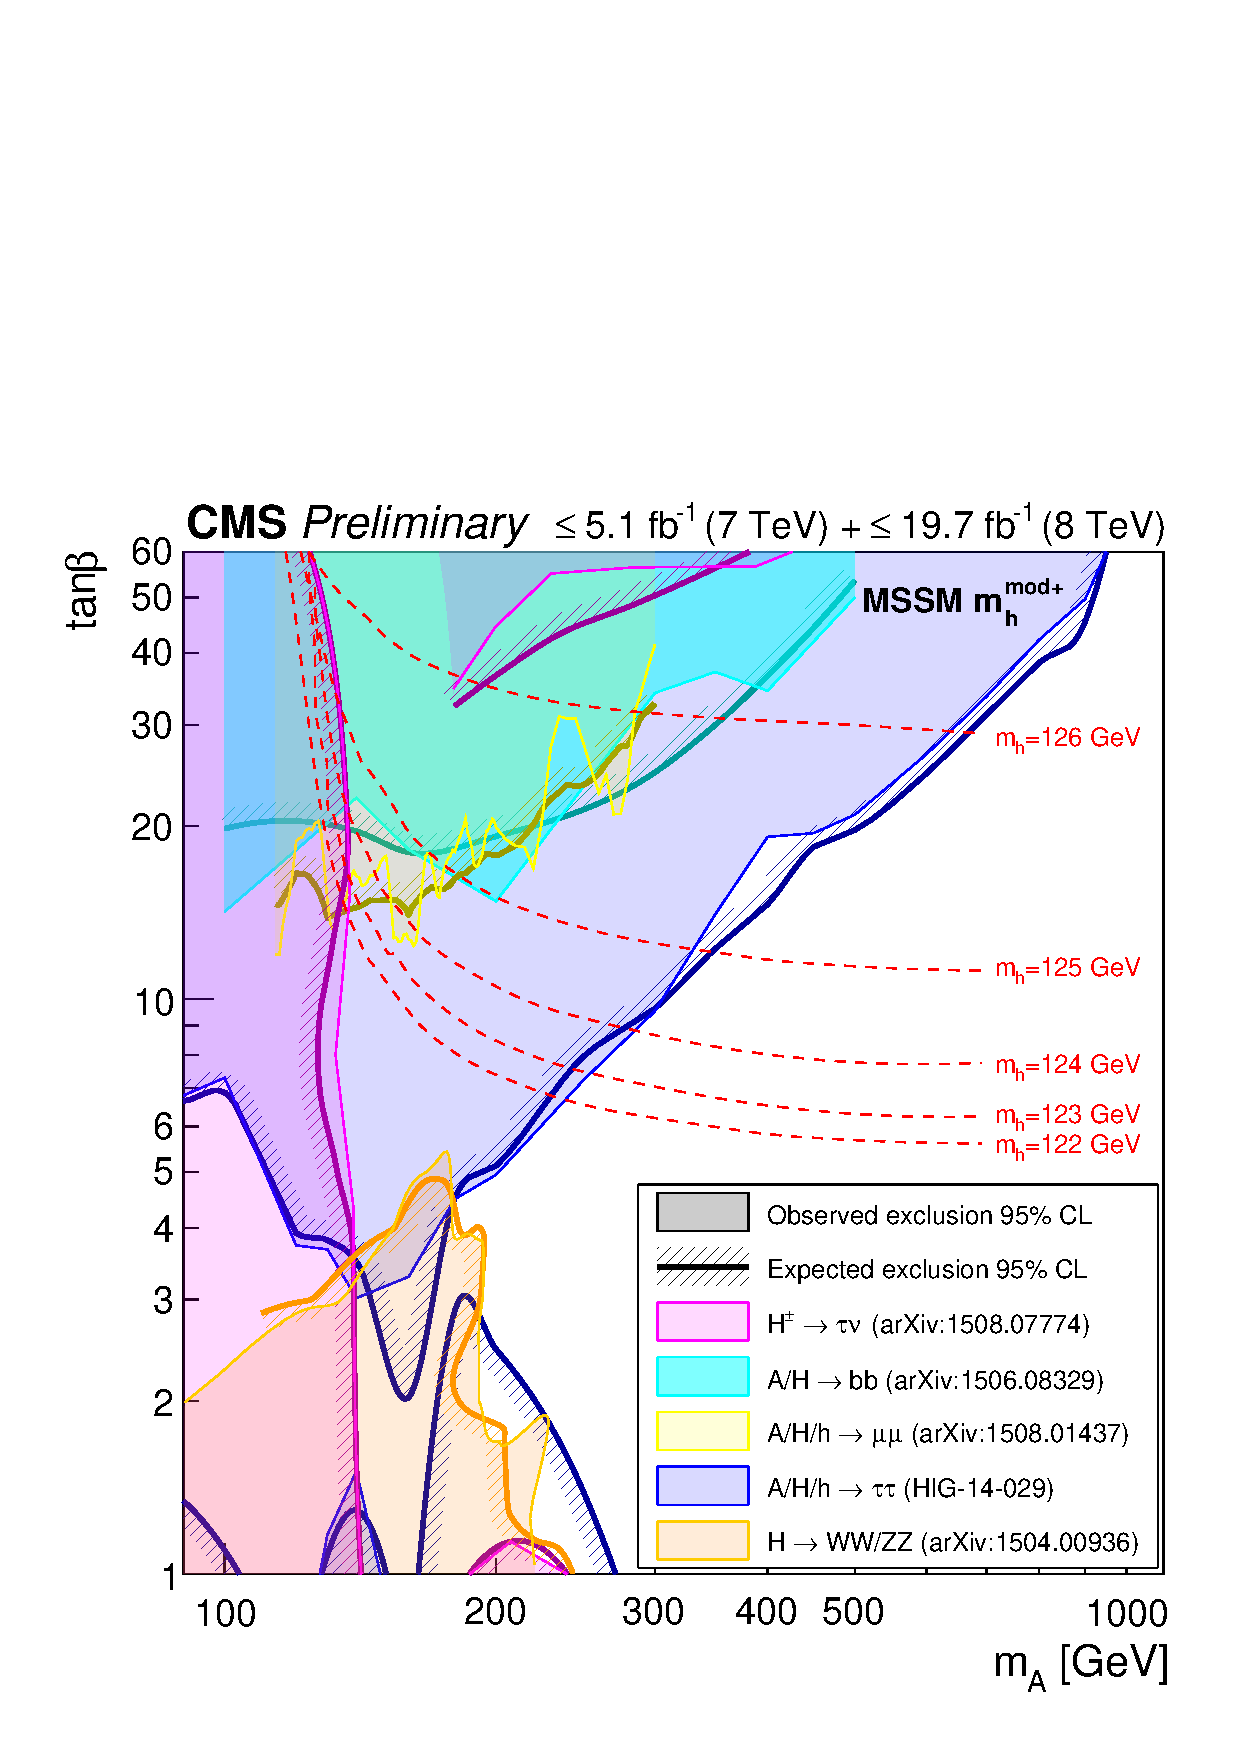
\includegraphics[width=0.5\textwidth]{./Theory/Figures/CMS-PAS-HIG-16-007_Figure_003-a.pdf}}
\subfloat[hMSSM scenario]{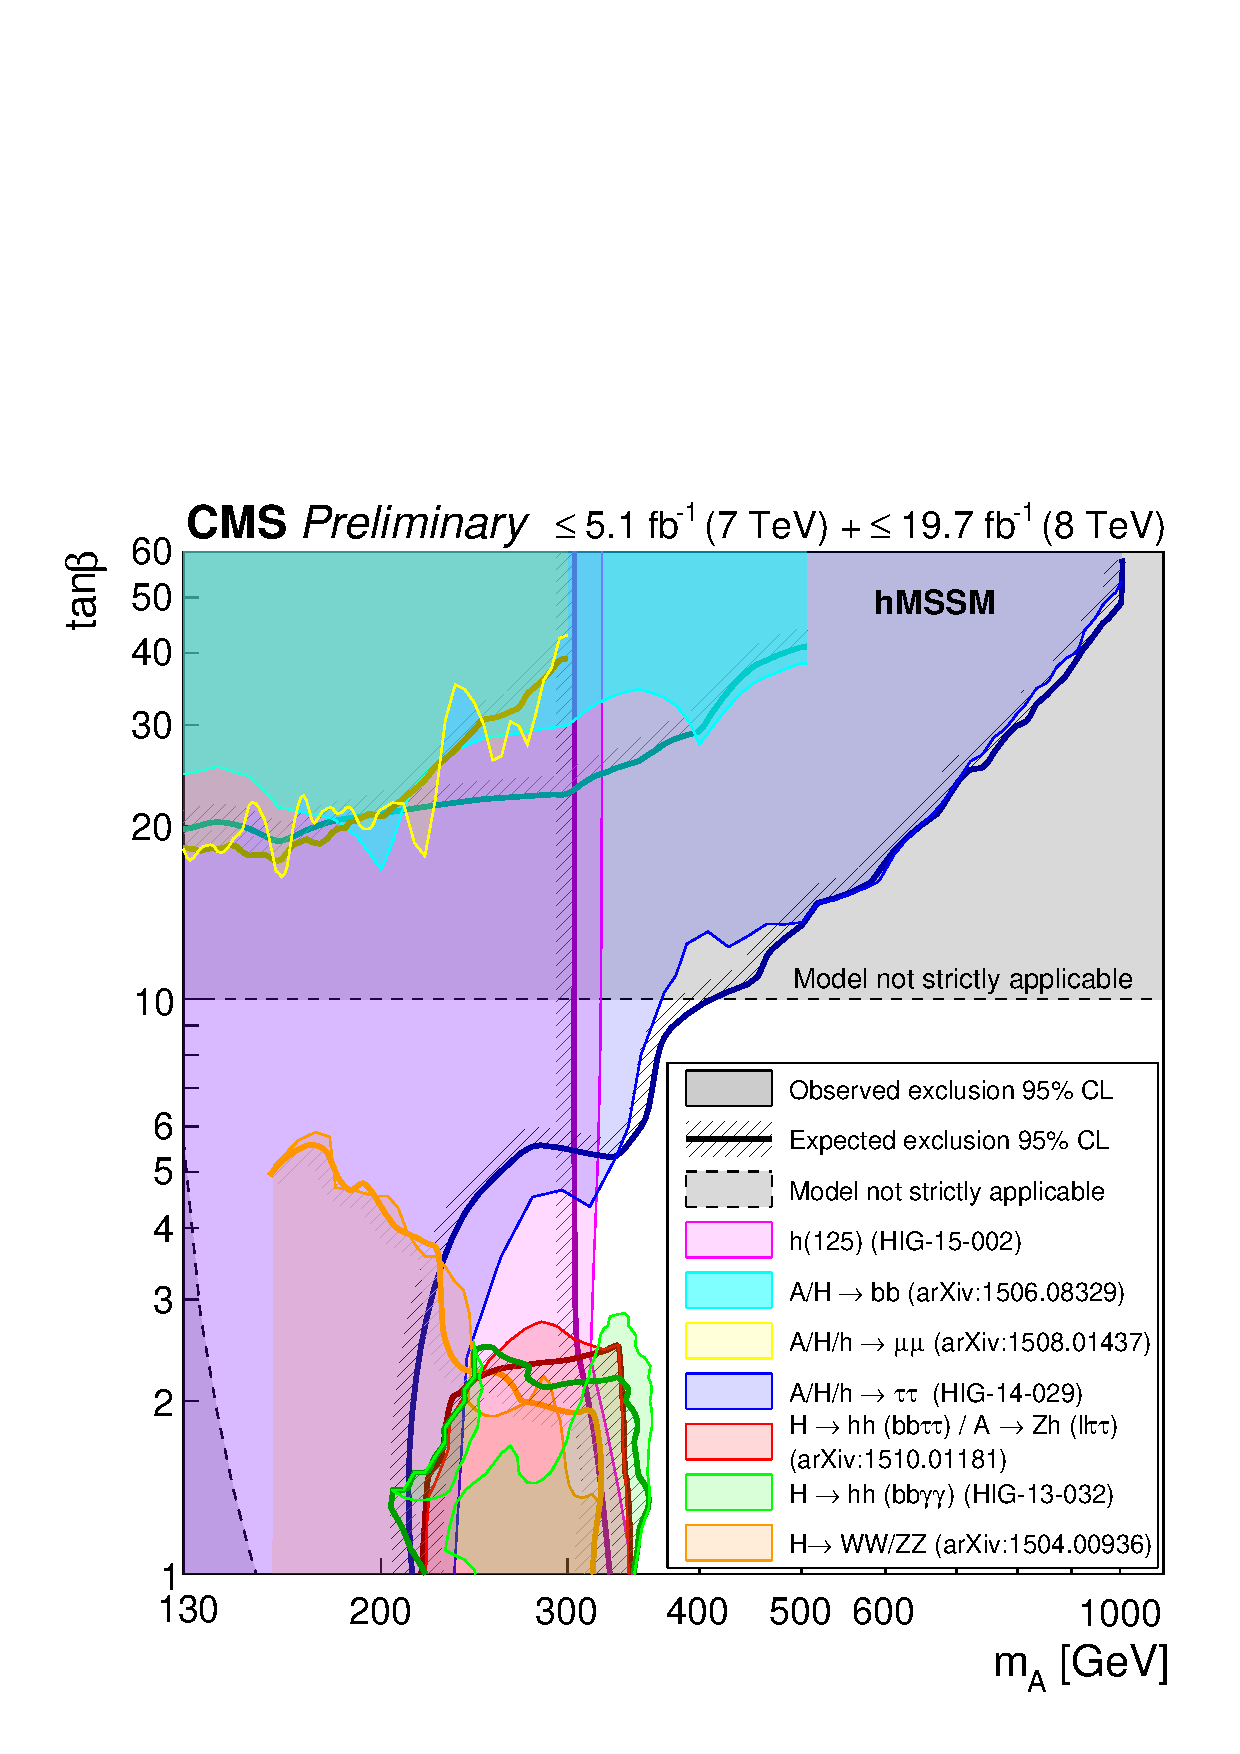
\includegraphics[width=0.5\textwidth]{./Theory/Figures/CMS-PAS-HIG-16-007_Figure_003-b.pdf}}
\end{center}
\caption{Summary of the interpretations of Run 1 BSM Higgs searches at \ac{CMS} in (a) the $m_{h}^{\text{mod+}}$ and (b) the
hMSSM scenario. The different coloured areas indicate the observed and expected exclusion from different searches in these
scenarios. The results from MSSM Higgs searches with decays into $\tau$ leptons are shown in blue and exclude more of the parameter
space than any of the other searches. The MSSM Higgs to $b\bar{b}$ (cyan) and Higgs to $\mu\mu$ (yellow) searches are also sensitive in part
of the high-\tanb region, with Higgs to WW or ZZ (orange) providing exclusion power at low \tanb~and low mass. In the $m_{h}^{\text{mod+}}$ 
scenario the charged Higgs to $\Pgt\Pgn$ search (magenta) excludes the low-mass region for all values of \tanb. Masses below around 300 GeV in the 
hMSSM scenario are excluded instead by constraints from standard model Higgs boson measurements (magenta). In this scenario small
areas of the low-\tanb~region are also excluded by the search for $H\rightarrow hh \rightarrow bb\tau\tau$ and $A\rightarrow Zh \rightarrow \ell\ell\tau\tau$ (red)
and the search for $H\rightarrow hh \rightarrow bb\gamma\gamma$ \cite{CMS-PAS-HIG-16-007}.}
\label{fig:bsm_summary}
\end{figure}


